%*******************************************************************************
%****************************** Third Chapter **********************************
%*******************************************************************************

\chapter{Methodology}

\ifpdf
    \graphicspath{{Chapter3/Figs/Raster/}{Chapter3/PDF/}{Chapter3/Figs/}{Figs/}}
\else
    \graphicspath{{Chapter3/Figs/Vector/}{Chapter3/Figs/}{Figs/}}
\fi

This chapter details the methodology guiding the system design, core features, software tools utilized, and the overall deployment and testing strategies employed for the University of San Carlos Patient Information System (USC-PIS). The development process follows a highly structured, user-centered engineering approach tailored to modernize the clinic's healthcare delivery.

\section{Conceptual Framework}

The conceptual framework for developing the USC-PIS (illustrated in Figure \ref{fig:conceptual_framework}) is anchored in a User-Centered Design (UCD) approach, which prioritizes the workflows of clinic staff and the accessibility needs of the students. The legacy system at the USC Clinic was heavily reliant on fragmented, paper-based records (such as the Daily Treatment Records) and basic Google Forms for feedback, which introduced significant inefficiencies in data retrieval and program evaluation.

\clearpage
\begin{figure}[!ht]
    \centering
    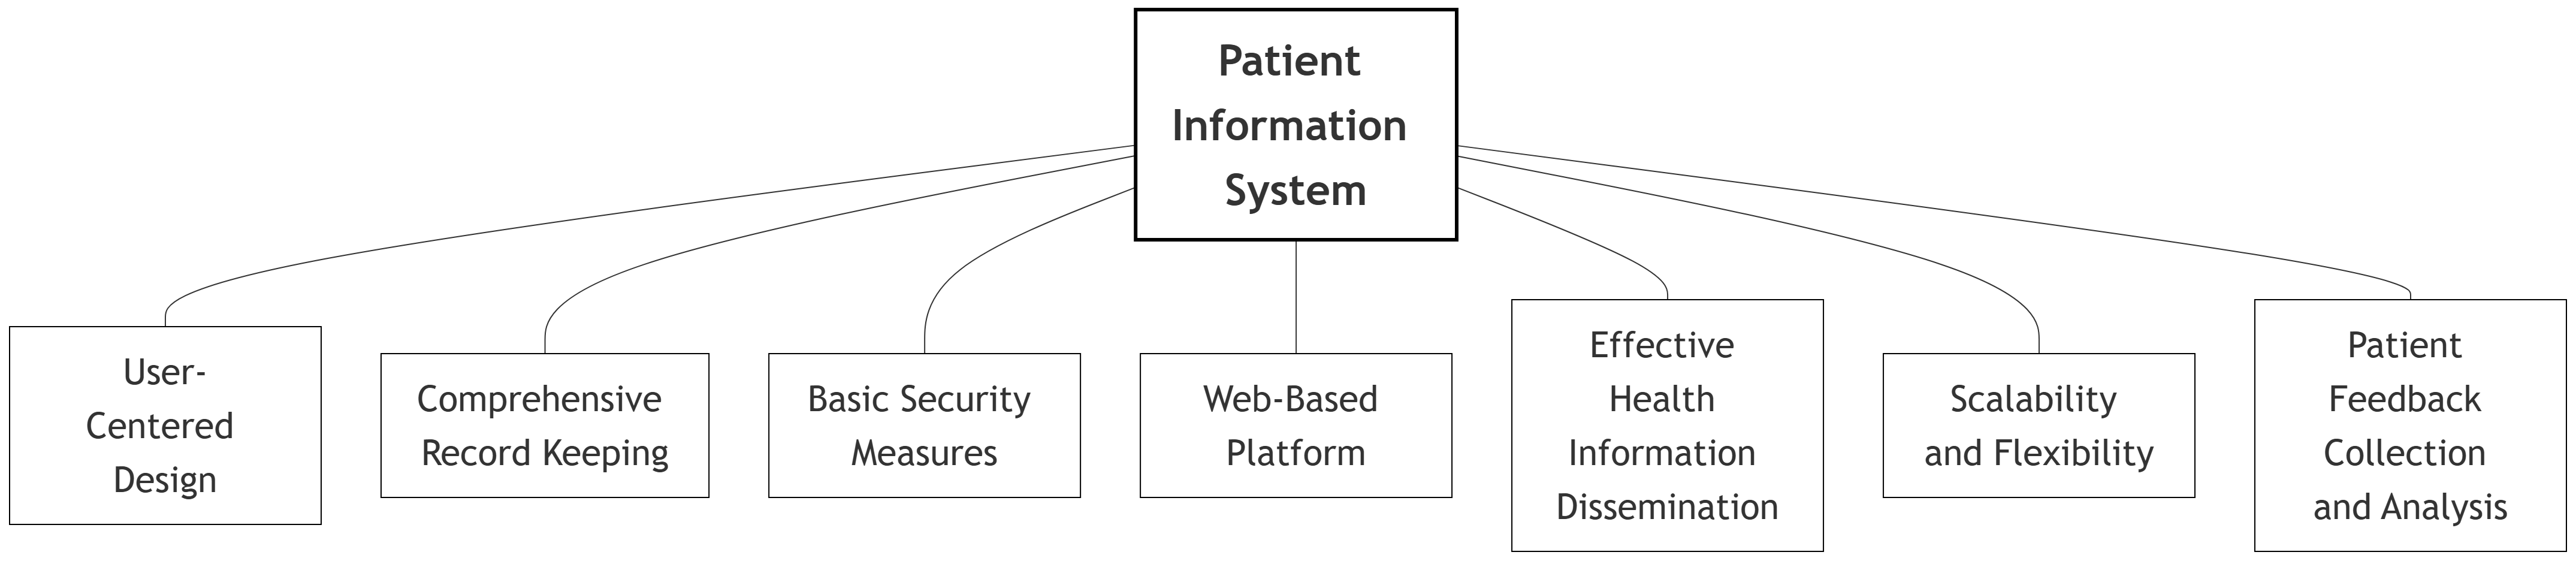
\includegraphics[width=0.9\textwidth]{ConceptualFramewor}
    \caption{Conceptual Framework of the USC-PIS}
    \label{fig:conceptual_framework}
\end{figure}
\clearpage

To resolve these bottlenecks, the modernized framework was constructed upon the following core pillars:

\begin{enumerate}
    \item \textbf{Comprehensive Record Keeping:} Centralizing medical histories and dental records in a secure database. This centralization was achieved by consolidating previously fragmented paper-based records into a unified digital repository. The system aggregates medical consultations, detailed dental records, and longitudinal health insights into a single patient-centric timeline, allowing clinical staff to access a complete and chronological view of a student's medical history without the need for manual cross-referencing across different physical files.
    \item \textbf{Effective Health Information Dissemination:} Utilizing dedicated digital campaigns to promote preventive care and health awareness across the campus.
    \item \textbf{Patient Feedback Collection and Analysis:} Integrating automated, digital evaluation forms following consultations to enable data-driven service refinement.
    \item \textbf{Basic Security Measures \& Privacy:} Enforcing robust data encryption and Role-Based Access Control (RBAC) to safeguard Protected Health Information (PHI).
\end{enumerate}

\section{Systems Analysis and Design}

\subsection{System Architecture}

The USC-PIS is engineered using a modern, scalable three-tier web architecture (illustrated in Figure \ref{fig:system_architecture}). This design ensures a clean separation of concerns, allowing for independent scaling and maintenance of the presentation, logic, and data storage components.

\clearpage
\begin{sidewaysfigure}
    \centering
    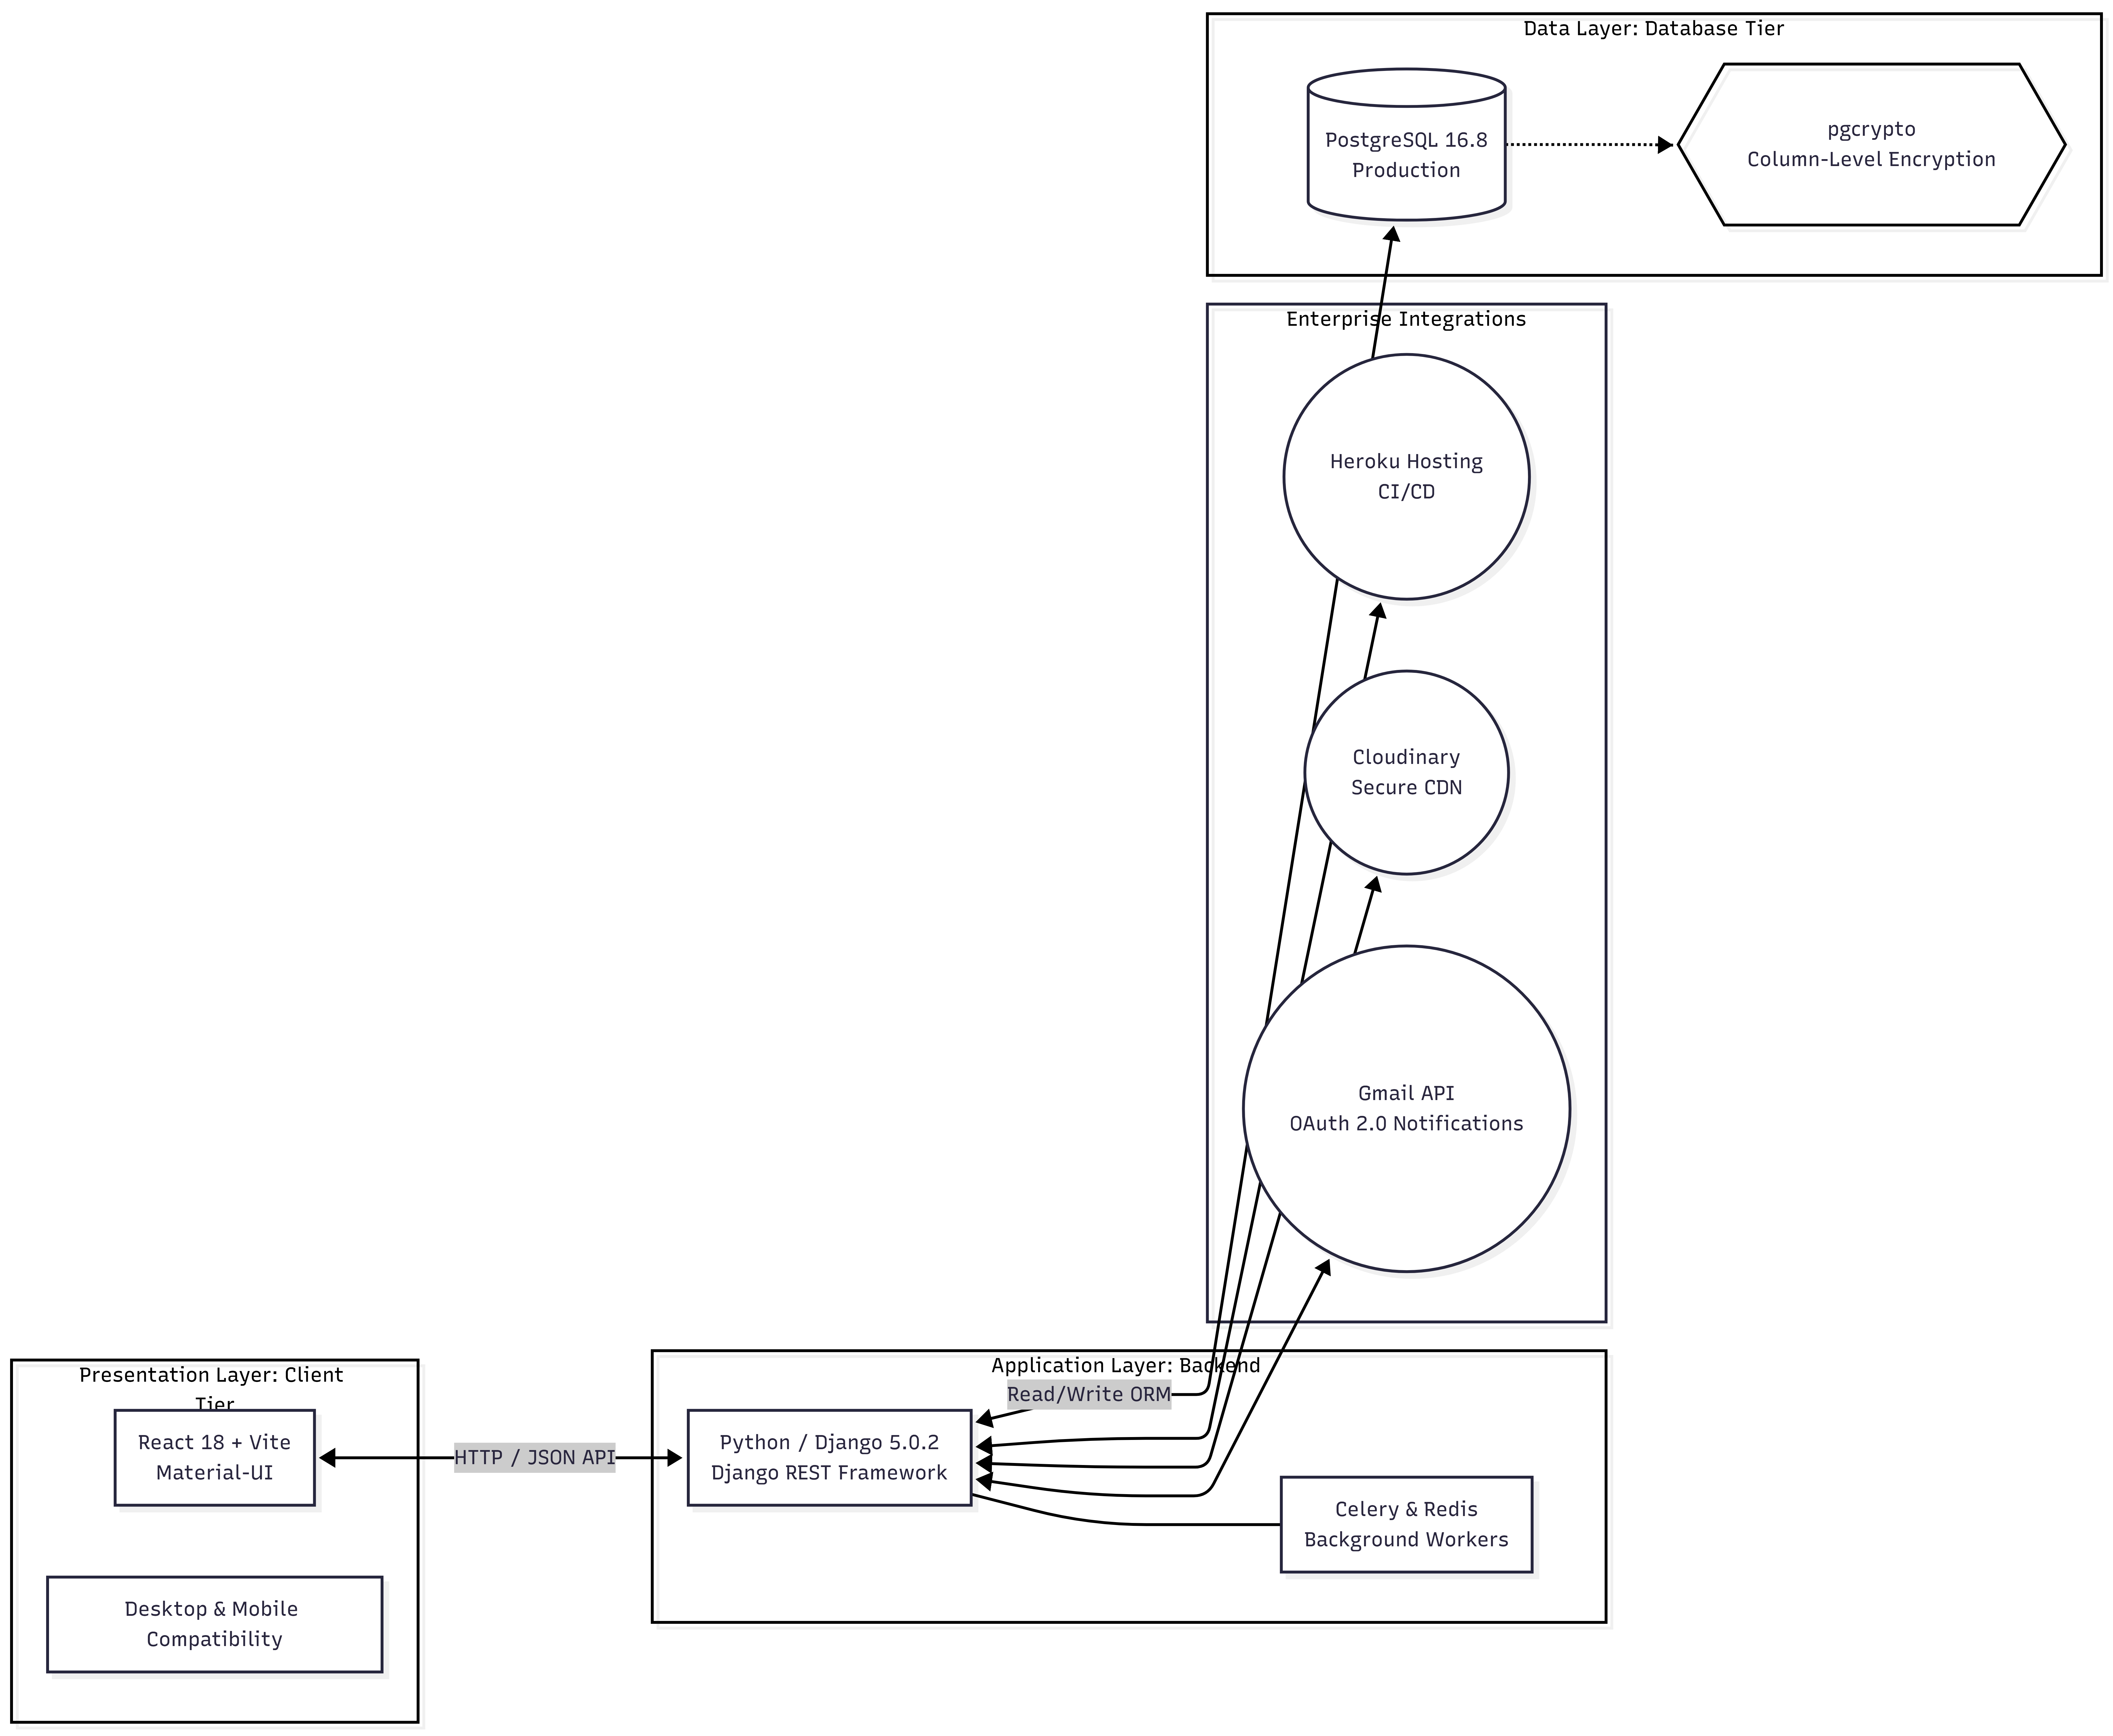
\includegraphics[width=0.9\textheight]{SystemArchitecture}
    \caption{Top-Level System Architecture of the USC-PIS}
    \label{fig:system_architecture}
\end{sidewaysfigure}
\clearpage

The architectural flow centers on the RESTful communication between the React frontend and the Django backend. As shown in the diagram, the backend serves as the central hub, managing secure data access to the PostgreSQL database while delegating time-consuming operations, such as PDF generation and automated email dispatch, to an asynchronous task queue managed by Celery and Redis.

\begin{itemize}
    \item \textbf{Presentation Layer (Frontend):} Developed using React 18 with a Vite build system and Material-UI components, providing a highly responsive and low-latency Graphical User Interface (GUI) across various devices.
    \item \textbf{Application Layer (Backend):} Powered by Python and Django 5.0.2, integrated with the Django REST Framework (DRF) 3.14.0. This layer handles business logic, automated notifications, and the system's strict RBAC middleware.
    \item \textbf{Data Layer (Database):} The system utilizes a dual-database paradigm: PostgreSQL 16.8 for production deployment and SQLite for local development, utilizing vendor-aware logic to ensure environment compatibility.
\end{itemize}

\section{System Workflows and Visual Analysis}

\subsection{Context Diagram}
The Context Diagram provides a high-level overview of the USC-PIS and its interactions with external entities. The system acts as the central hub bridging the clinical staff and the student body. Students interact with the platform to access their personal health information and submit visit-linked feedback, while Clinic Staff (Doctors, Nurses, and Dentists) input clinical data, issue medical certificates, and manage health campaigns. All transactions are routed securely to the central Patient Database, ensuring real-time data synchronization across all user endpoints.

\clearpage
\begin{figure}[!ht]
    \centering
    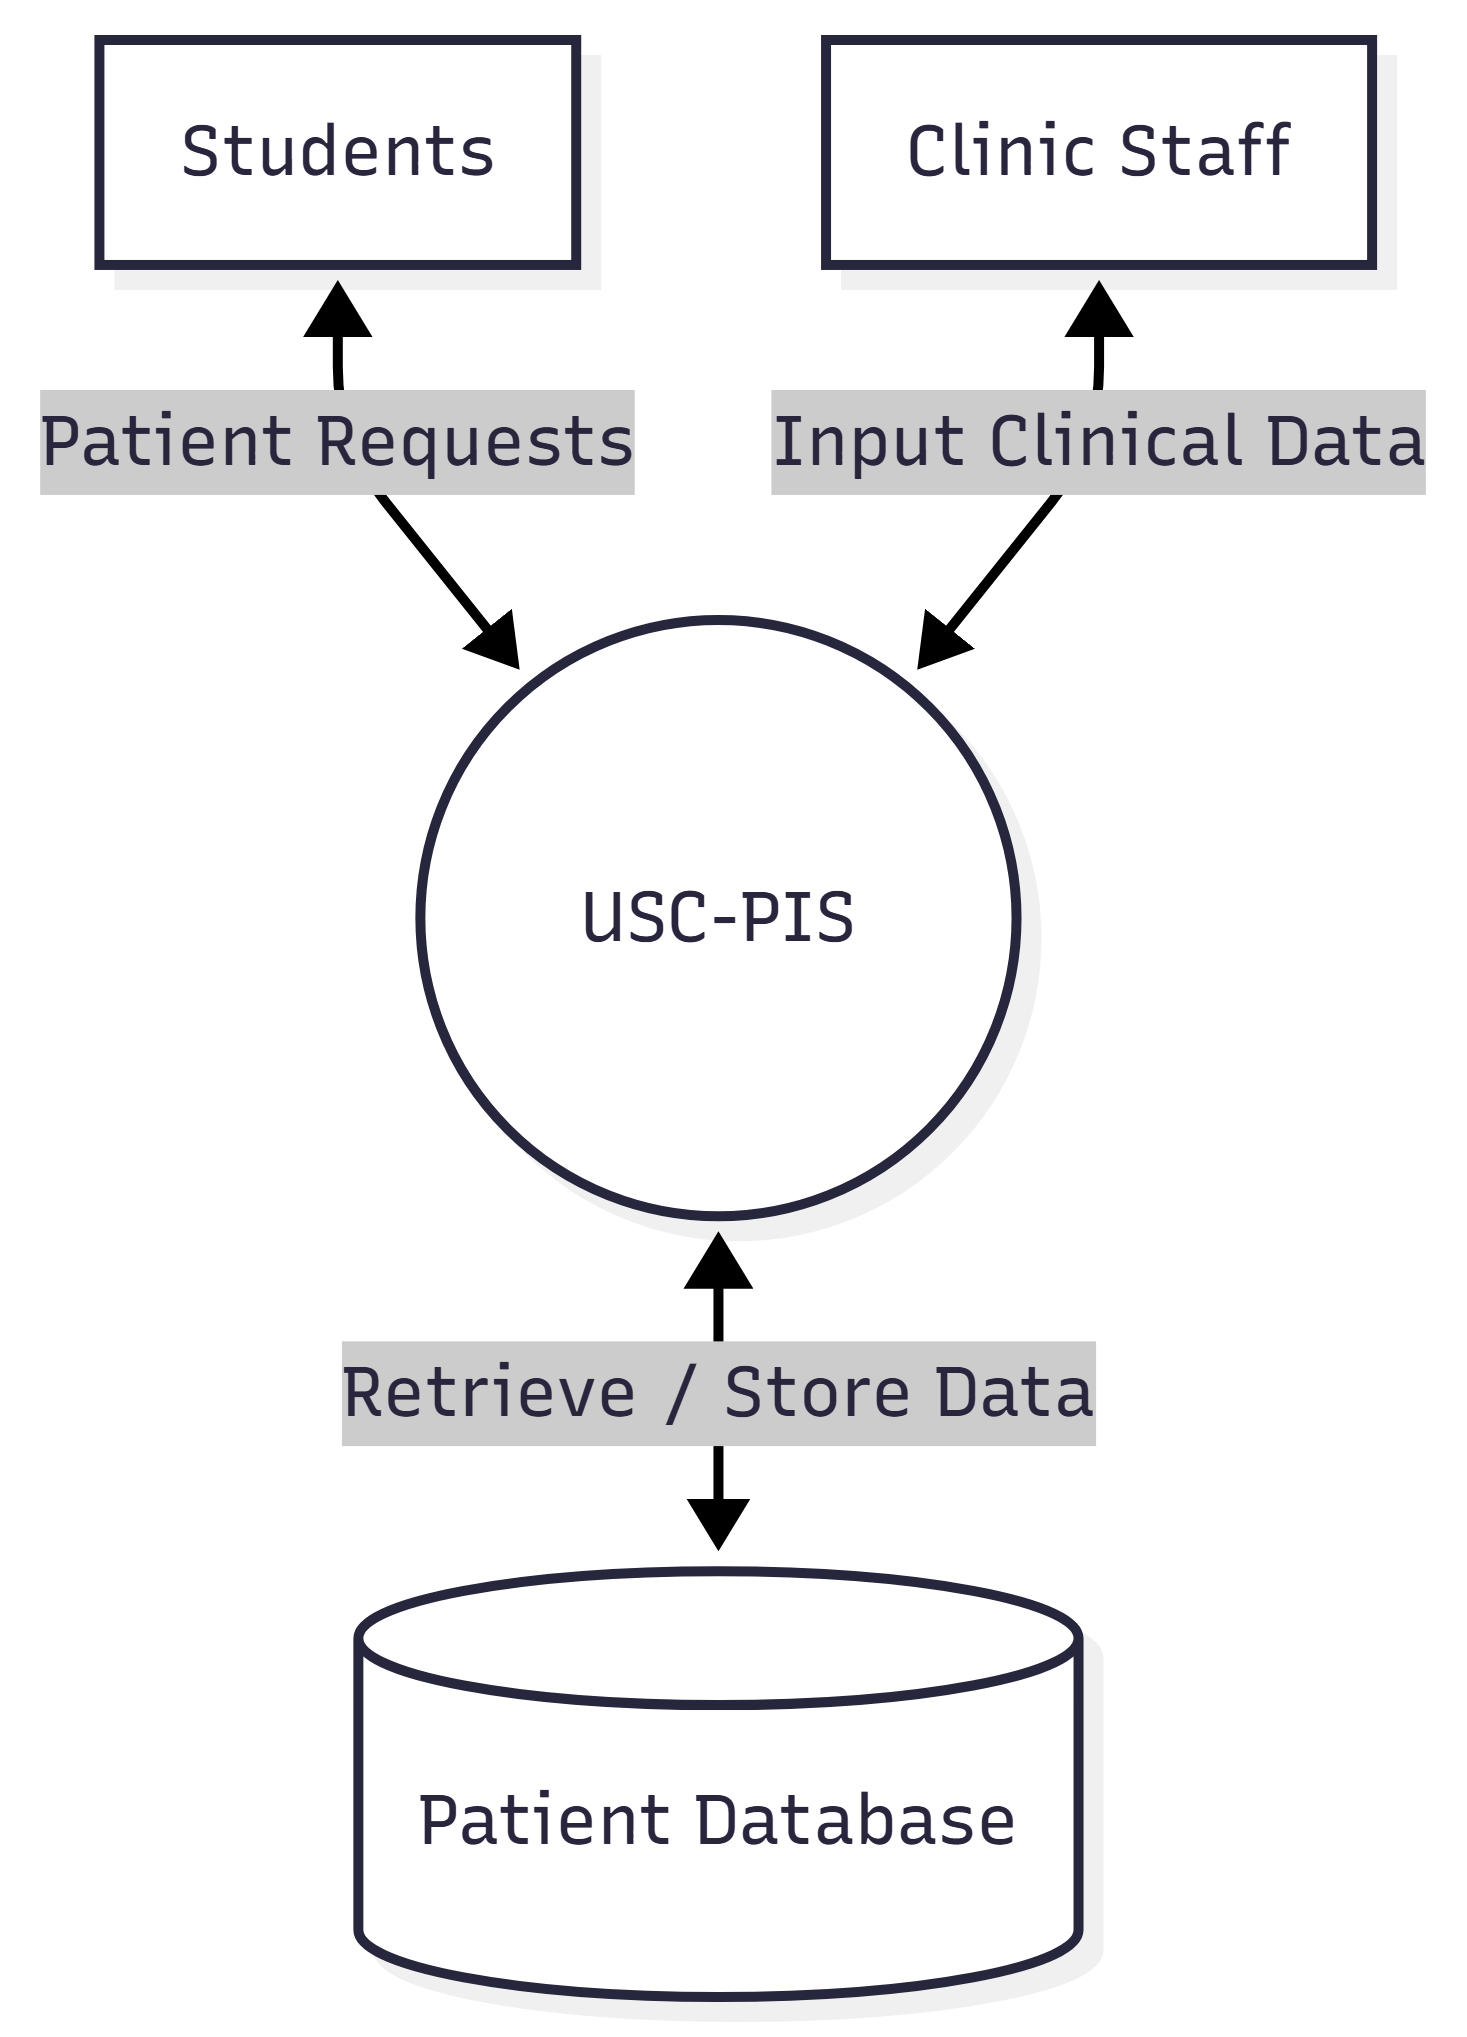
\includegraphics[width=0.95\textwidth]{ContextDiagram}
    \caption{Context Diagram of the USC-PIS}
    \label{fig:context_diagram}
\end{figure}
\clearpage

\subsection{User Roles and Functionalities}
To safeguard Protected Health Information (PHI) and Personally Identifiable Information (PII), the USC-PIS employs a strict Role-Based Access Control (RBAC) architecture enforced via Django REST Framework (DRF) permission classes. Notably, all professional clinical roles (Admin, Doctor, Dentist, Nurse, and Staff) possess the authorization to create and export reports, while the System Audit Report is strictly reserved for the Admin role. The system dynamically restricts other access and capabilities across the following hierarchical user classes:

\begin{itemize}
    \item \textbf{Admin:} Possesses global system access, which includes managing RBAC adjustments, monitoring system health, administering the email notification system, and generating system audit reports. Crucially, the Admin role includes a comprehensive \textbf{Audit Logging} dashboard that tracks all system activities and data mutations (CREATE, UPDATE, DELETE), providing a full audit trail beyond simple log-in tracking.
    \item \textbf{Doctor and Dentist:} Both roles are endowed with full clinical and administrative access, allowing them to diagnose, prescribe treatments, access all feedback analytics, and generate clinical reports. For the \textbf{Dentist} role, irrelevant medical fields are dynamically disabled to streamline the dental workflow, and a dedicated \textbf{Visual Dental Record Interface} is included for precise oral geography mapping.
    \item \textbf{Nurse:} Functions in a supervisory and clinical data-entry capacity. Nurses are authorized to manage patient intake, record vital signs, input treatment plans, generate clinical reports, and draft medical certificates (which remain pending until Doctor issuance).
    \item \textbf{Staff:} Responsible for clinic administration. This role manages patient intake processing, certificate issuance, clinical report generation, and the creation and deployment of health awareness campaigns.
    \item \textbf{Student and Faculty (Patient):} This role is restricted strictly to their own data. Patients are only permitted to view their personal medical and dental timelines via the Health Insights dashboard, submit visit-linked feedback, and view public health campaigns.
\end{itemize}

The system also integrates a multi-tiered \textbf{System Alerts} architecture, providing real-time notifications, prompts, and visual alerts for all data changes and important clinical updates across the interface.

\subsection{Authentication Workflow}
The authentication sequence is designed to ensure stringent identity verification before granting system access while maintaining high data consistency. To eliminate manual input errors, USC ID numbers are auto-captured from the institutional database, and user roles are automatically assigned based on their verified status upon registration. Furthermore, the system implements a streamlined GMail auto sign-in mechanism to reduce friction. The sequential workflow begins with a student registering an account, where the system actively enforces a domain constraint, requiring the email to end in \texttt{@usc.edu.ph}. Upon validation, the Django backend generates a 6-digit One-Time Password (OTP) with a precise 10-minute expiration window. This OTP is transmitted to the user via the Gmail API OAuth 2.0 integration. Once the user inputs the correct OTP, the system authenticates the session and issues a secure JWT token, granting access to the role-gated dashboards.

\clearpage
\begin{figure}[!ht]
    \centering
    \makebox[\textwidth][c]{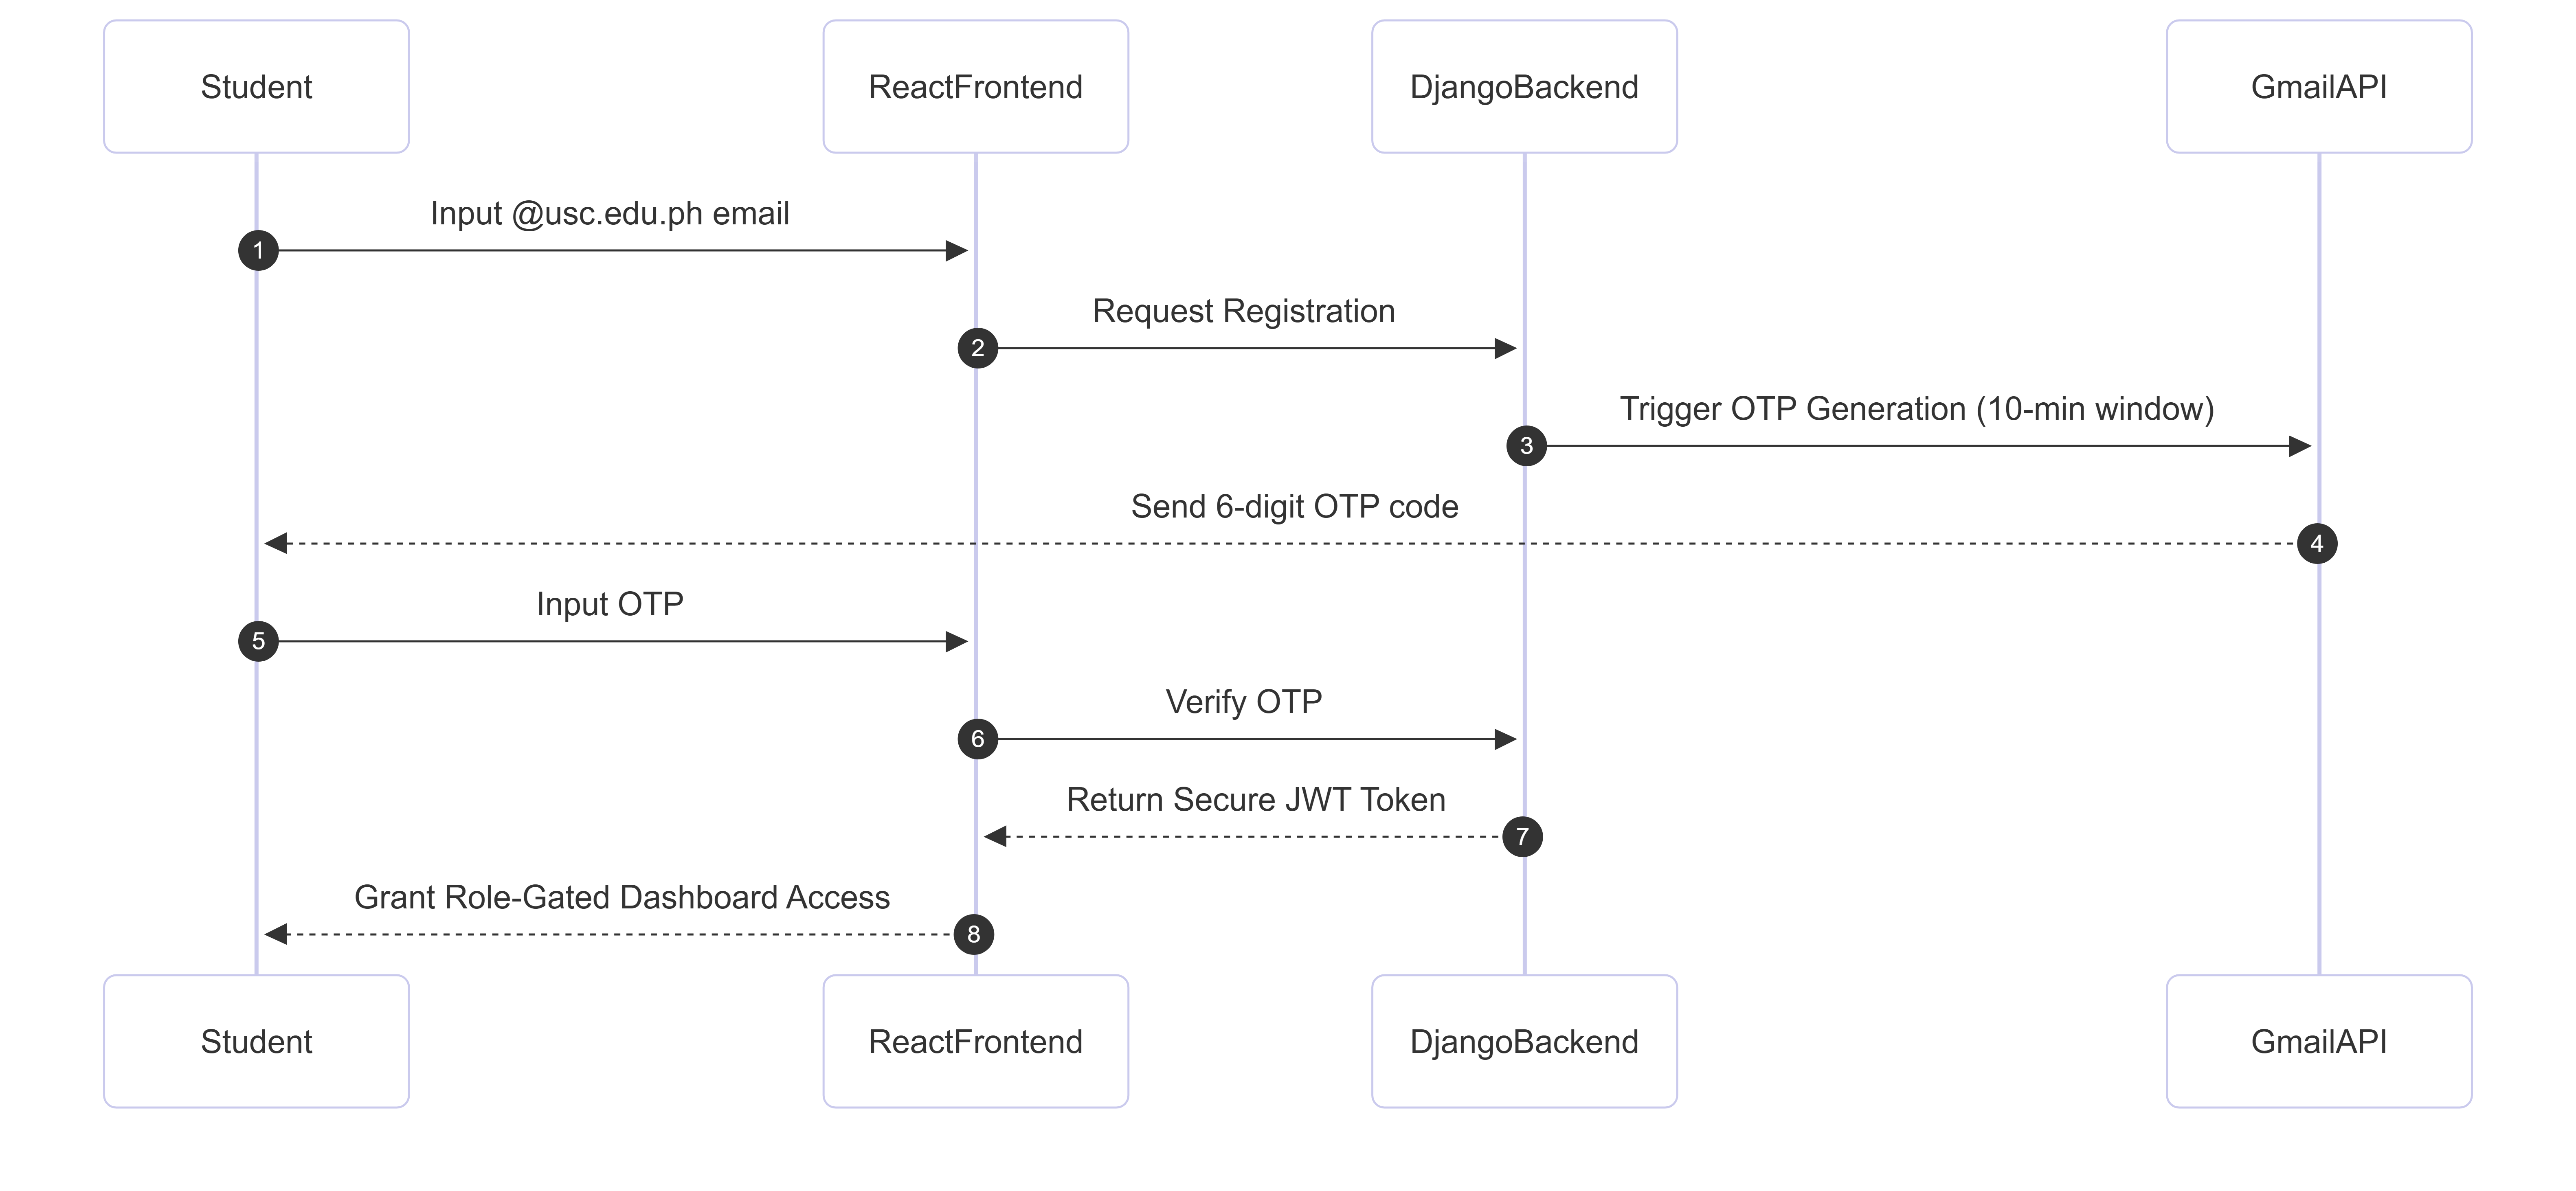
\includegraphics[width=1.25\textwidth]{AuthenticationWorkflow}}
    \caption{Sequential Authentication Workflow of the USC-PIS}
    \label{fig:authentication_workflow}
\end{figure}
\clearpage

\subsection{Clinical Record and Security Pipeline}
To comply with strict data privacy mandates, the USC-PIS employs a highly secure data flow pipeline for clinical records. When medical personnel utilize the Unified Record Component to enter vital signs and a clinical diagnosis, the data is transmitted to the Application Layer. Before the data is committed to the PostgreSQL database, a Django \texttt{post\_save} signal intercepts the transaction. This signal executes the \texttt{pgp\_sym\_encrypt} function, instantly converting plaintext Protected Health Information (PHI), such as patient names and diagnoses, into secure \texttt{BinaryField} (\texttt{bytea}) hashes. This ensures military-grade encryption-at-rest with minimal computational overhead. To maintain clinical data integrity, the pipeline includes robust \textbf{Validation and Error Trapping} mechanisms. The system autonomously calculates BMI based on height and weight inputs, traps dates to block impossible future dates for birthdays or visit records, and validates erroneous clinical inputs such as negative temperatures or zero blood pressure readings to prevent data entry errors.

Furthermore, the system incorporates an \textbf{Attributed Clinical Remarks System} to enhance inter-professional collaboration. This feature allows Doctors to view historical remarks and clinical notes authored by other medical personnel during patient consultations. By providing a centralized, color-coded view of previous clinical observations, the system ensures collaborative care and seamless coordination between different healthcare providers, allowing for a more informed and comprehensive assessment of the patient's medical history.

\clearpage
\begin{sidewaysfigure}
    \centering
    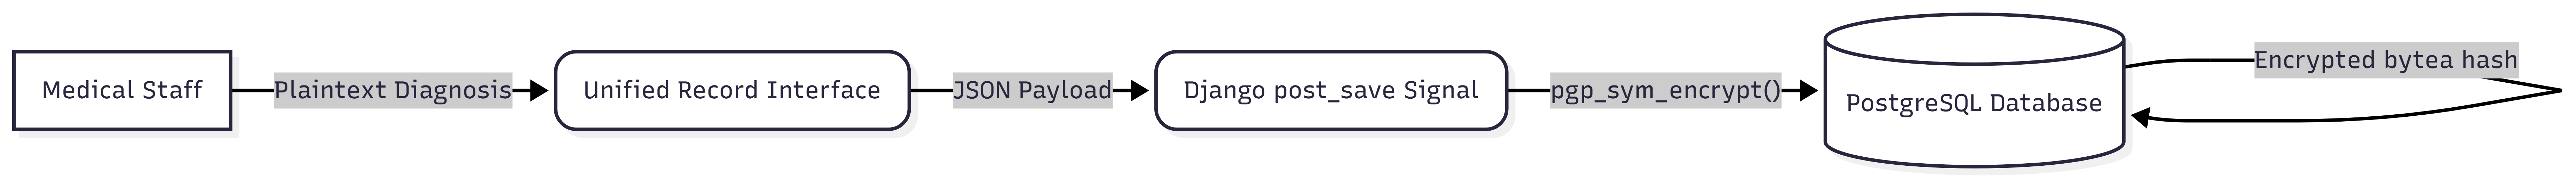
\includegraphics[width=1.0\textheight]{ClinicalRecordSecurityPipeline}
    \caption{Clinical Record Data Flow and Security Pipeline}
    \label{fig:clinical_record_pipeline}
\end{sidewaysfigure}
\clearpage

\subsection{The Medical Certificate Pipeline}
The issuance of the USC Form ACA-HSD-04F Medical Certificate follows a digitized, role-gated sequential pipeline. The workflow initiates when a Nurse or Staff member accesses a patient's record to draft the certificate and input the ``Purpose/Requirement''. However, the system's RBAC middleware restricts the rendering of the document until a user with the DOCTOR role assesses the draft. The Doctor must select the Medical Fitness Status (strictly displaying either ``Physically Fit'' or ``Unfit'', but never both) and authorize the issuance. Once the \texttt{IsDoctorUser} permission is validated, the system logs the issuance of the certificate along with the name of the issuing doctor. The backend dual-engine PDF module then autonomously renders the landscape-formatted certificate for download. To maintain administrative integrity, editing of rejected certificate requests is not allowed. For the student demographic, the interface displays the status as ``Ready to be Claimed'', as they cannot print the official document themselves.

\clearpage
\begin{figure}[!ht]
    \centering
    \makebox[\textwidth][c]{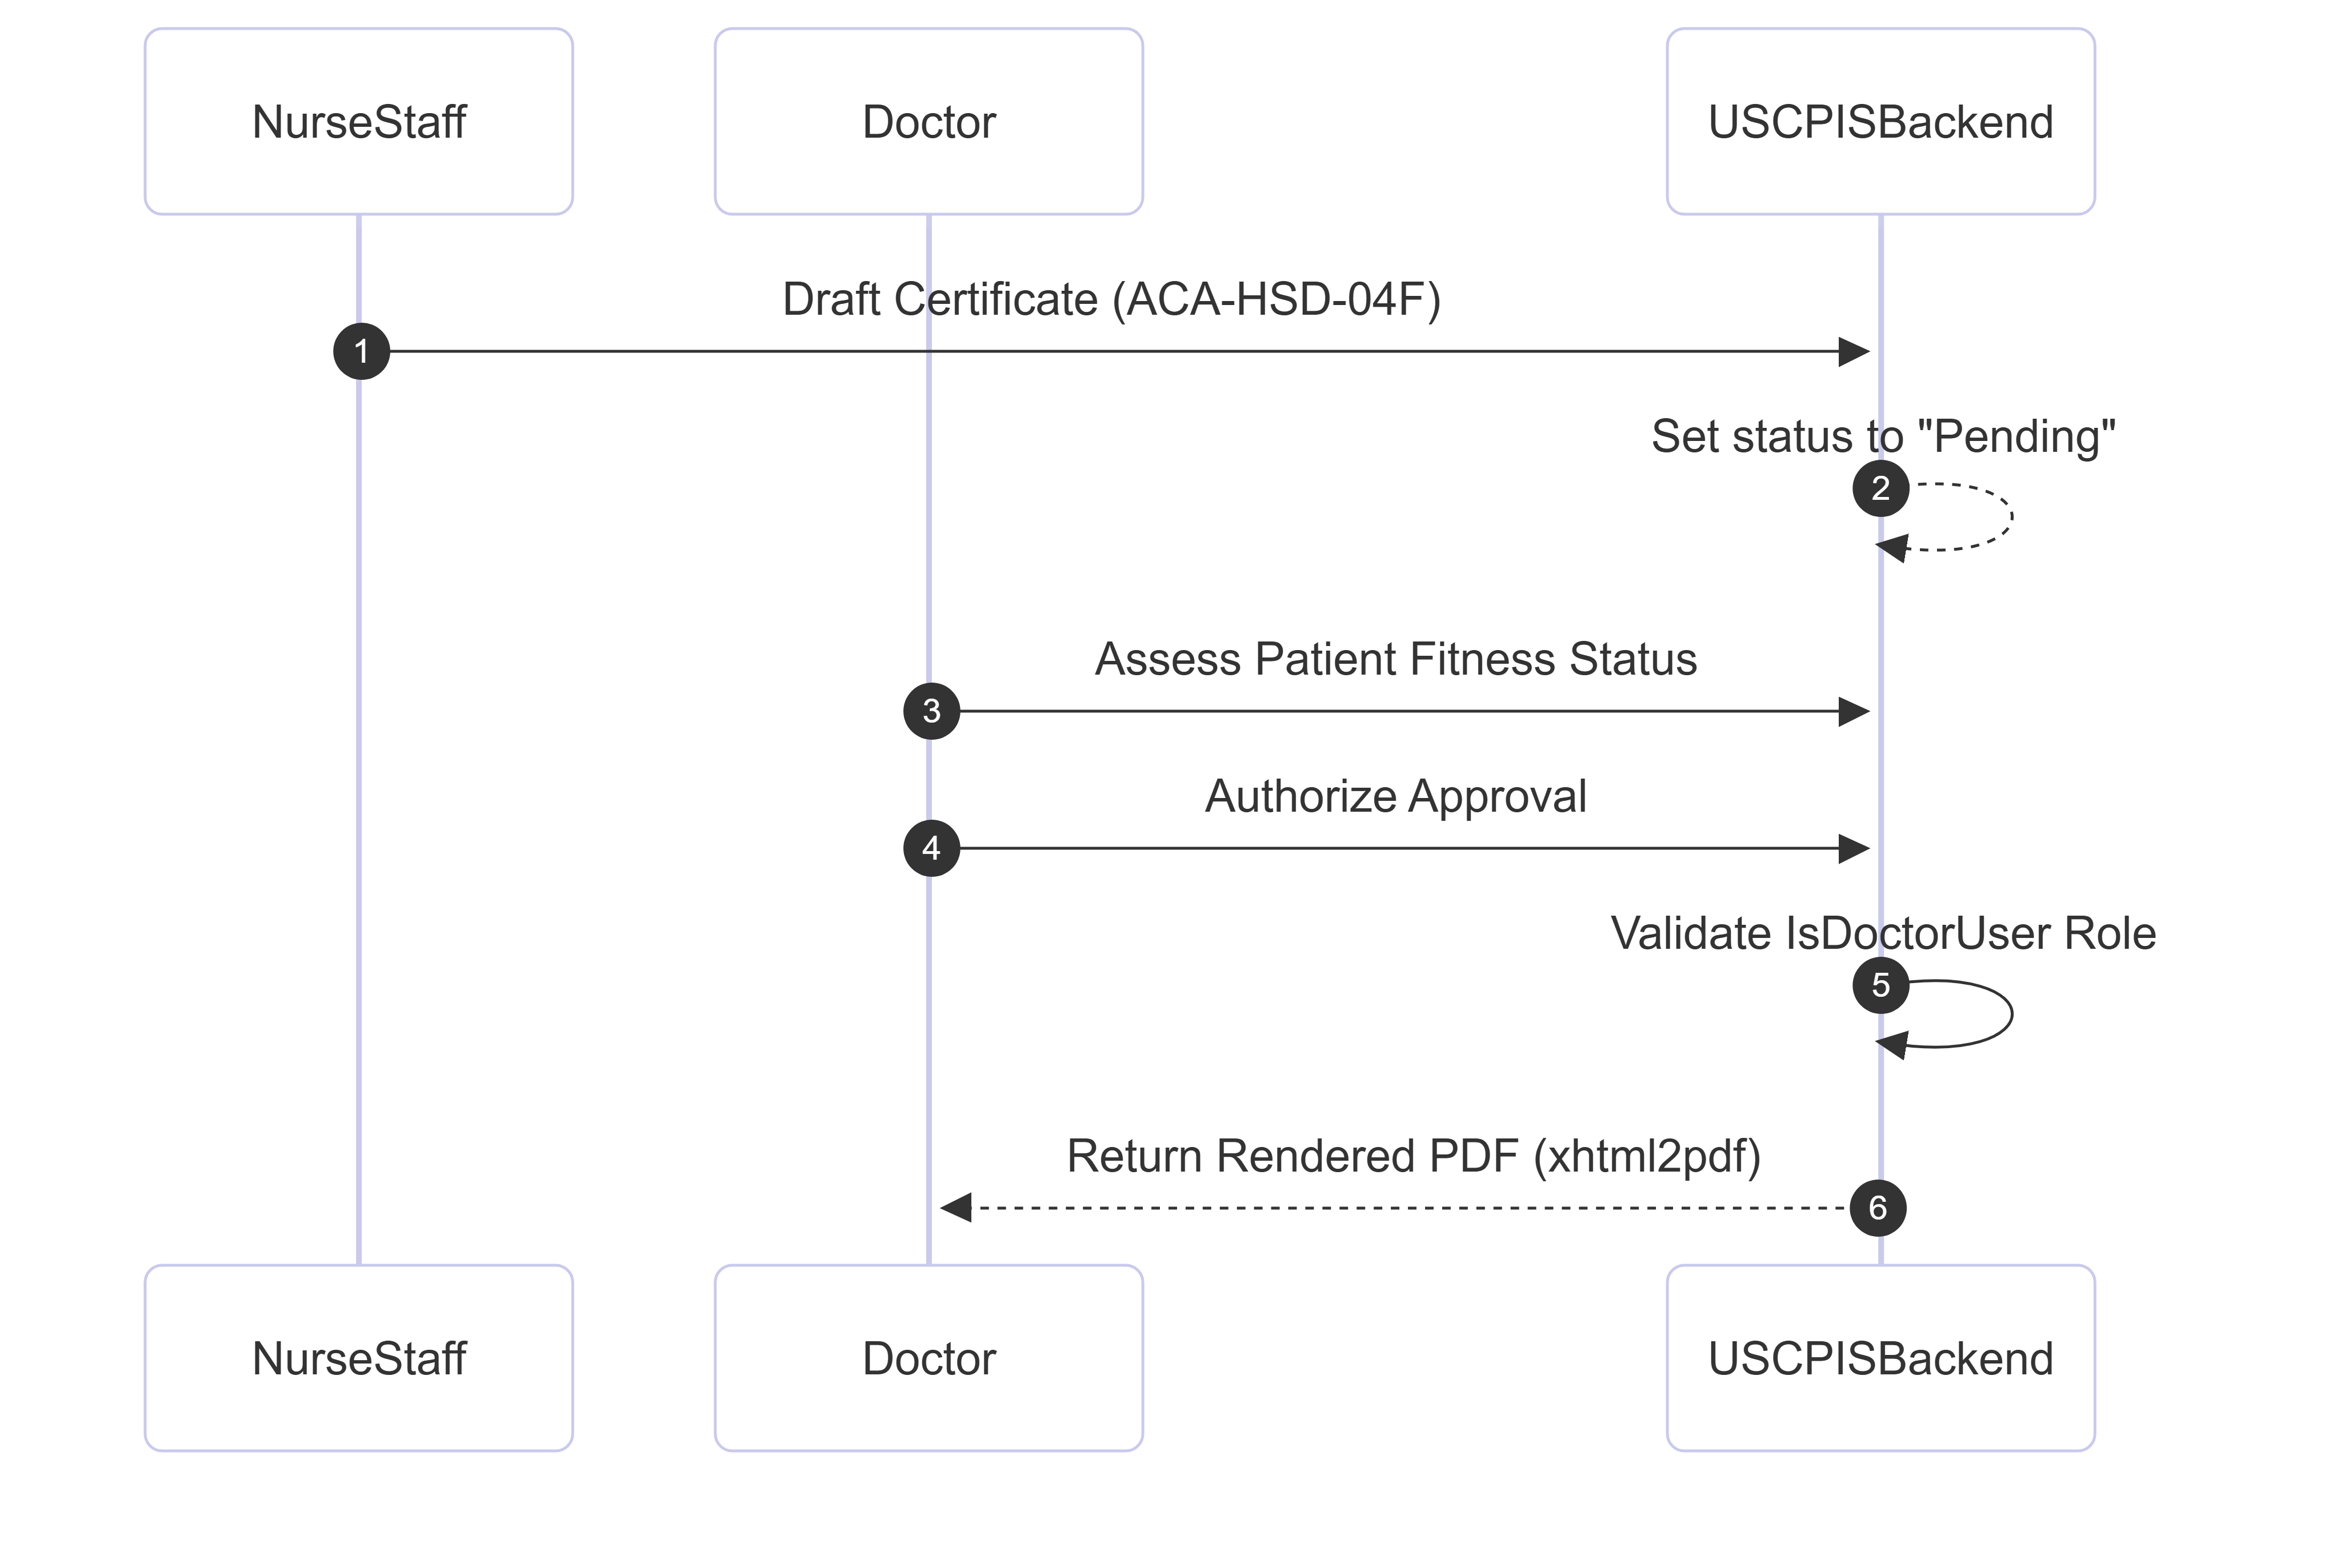
\includegraphics[width=1.25\textwidth]{MedicalCertificatePipeline}}
    \caption{Role-Gated Medical Certificate Issuance Pipeline}
    \label{fig:medical_certificate_pipeline}
\end{figure}
\clearpage

\section{Software Tools and Technology Stack}
The USC-PIS is engineered upon a modern, highly scalable three-tier web architecture designed to ensure a clean separation of concerns.

\begin{itemize}
    \item \textbf{Presentation Layer (Frontend):} The client-side interface was developed utilizing React 18 with a Vite build system and Material-UI components. This combination provides a responsive, low-latency, and component-based Graphical User Interface (GUI) that seamlessly adapts to both desktop and mobile environments for clinic staff and patients.
    \item \textbf{Application Layer (Backend):} The server-side logic is powered by Python and Django 5.0.2, deeply integrated with the Django REST Framework (DRF) 3.14.0. This layer encapsulates the core clinical business logic, API routing, and the Role-Based Access Control (RBAC) middleware that globally restricts endpoint access based on user classes. Notably, all professional clinical roles possess the authorization to create and export reports. Heavy data aggregations, such as the synthesis of clinic reports, are processed asynchronously via Celery and Redis background workers to prevent HTTP thread blocking. These reports now include interactive charts and graphs with fixed formatting and support dynamic filtering (e.g., filtering patient reports by school, course, or year level; feedback reports by rating; and campaign reports by type). Medical-related reports are specifically tailored to display all relevant clinical information required for administrative review.
    \item \textbf{Data Layer (Database):} The system operates on a dual-database paradigm, utilizing PostgreSQL 16.8 for production deployment and SQLite for local development. The PostgreSQL database natively integrates the \texttt{pgcrypto} extension to enforce column-level symmetric encryption for all Protected Health Information (PHI).
    \item \textbf{Enterprise Integrations:} The platform relies on Heroku for continuous deployment and hosting, Cloudinary for scalable Content Delivery Network (CDN) file storage (handling attachments and PubMats), and the Gmail API utilizing OAuth 2.0 to dispatch automated post-visit evaluations and authentication codes.
\end{itemize}

\section{Graphical User Interface (GUI) Design}
The Presentation Layer of the USC-PIS was engineered to be highly intuitive and responsive, minimizing the learning curve for both clinical staff and the student body. Built utilizing React 18, a Vite build system, and Material-UI (MUI) components, the interface strictly adheres to a clean, healthcare-appropriate aesthetic. The web application was rigorously checked for front-end errors and optimized for full mobile responsiveness. Furthermore, all specific visual corrections identified in the panel's annotated screenshots have been fully resolved to ensure a polished user experience.

\begin{figure}[!ht]
    \centering
    \makebox[\textwidth][c]{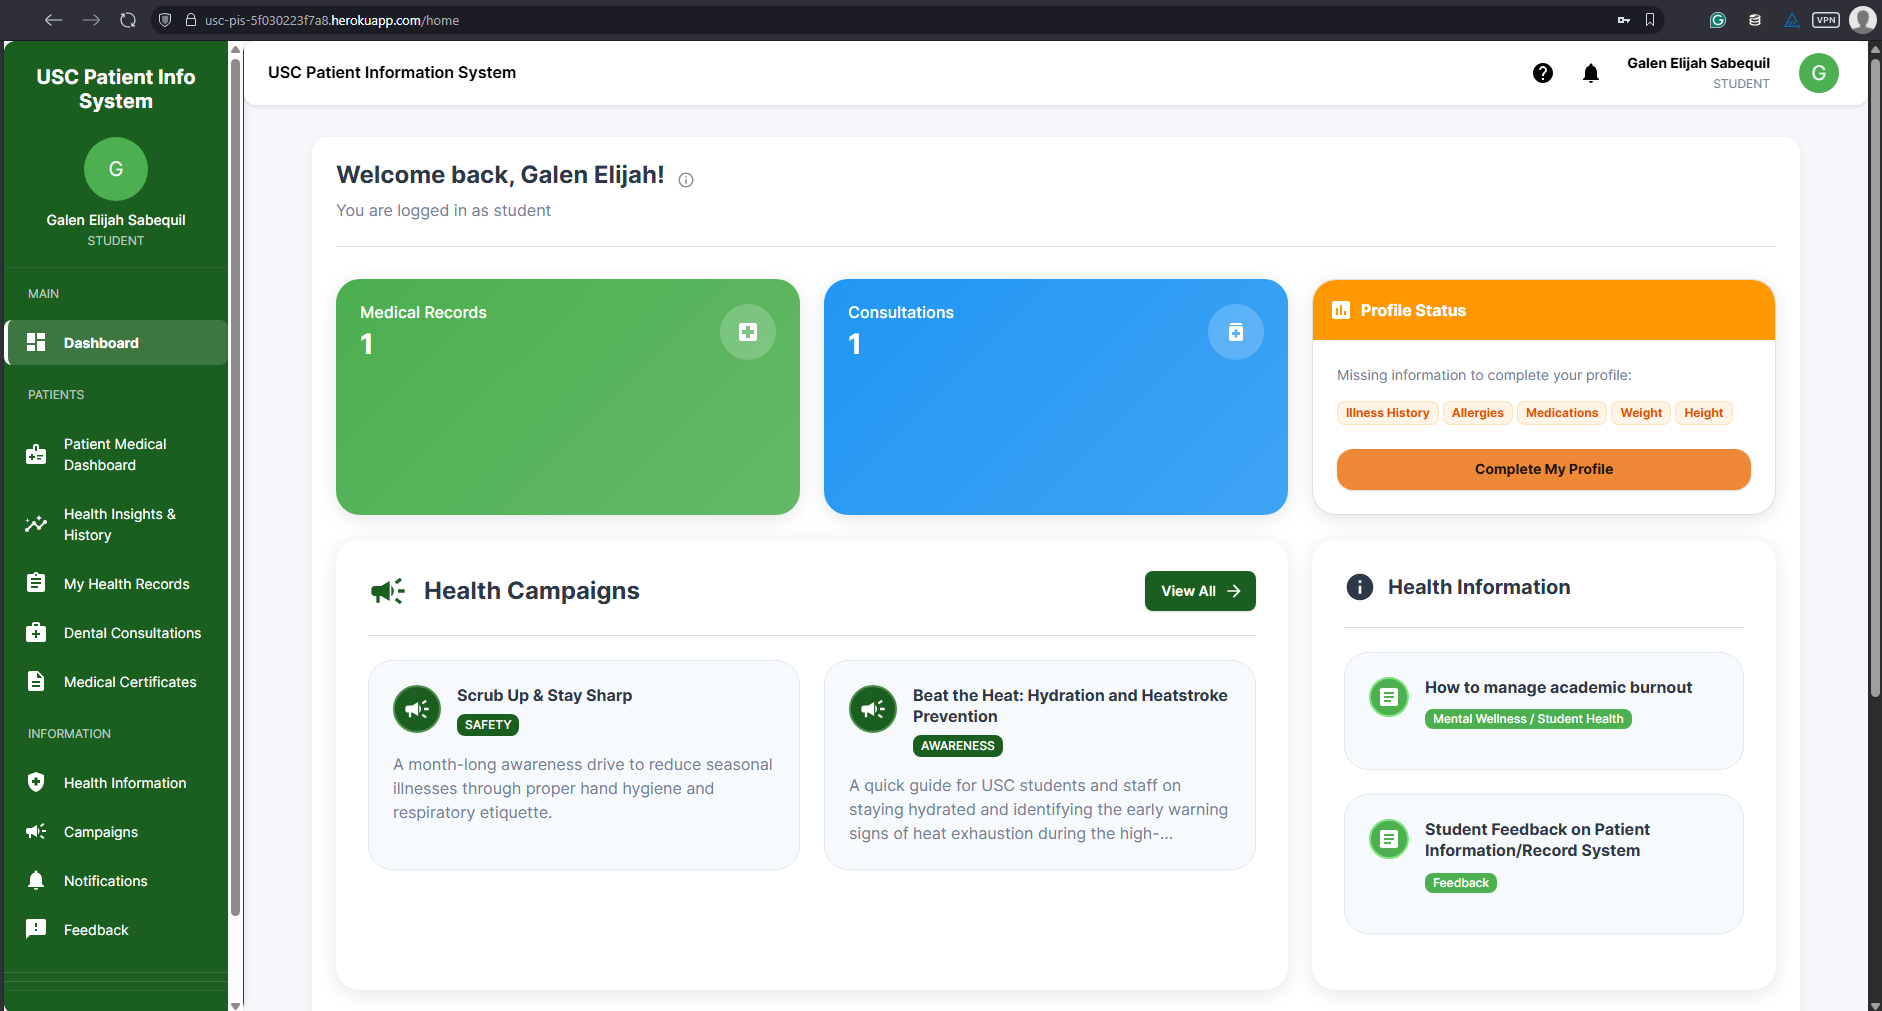
\includegraphics[width=1.1\textwidth]{WebsiteHomeDashboard}}
    \caption{The USC-PIS Home Dashboard Overview}
    \label{fig:home_dashboard}
\end{figure}

The interface employs progressive disclosure and a component-based architecture to adapt seamlessly to both desktop and mobile environments. To visually document the system's frontend capabilities, the following key interfaces were captured:

\subsection{The Patient Medical Dashboard}
The student-facing dashboard was designed to provide personalized health analytics. It features real-time counts of medical records and consultations, a 6-month visit frequency analysis, and automated BMI calculations.

\begin{figure}[!ht]
    \centering
    \makebox[\textwidth][c]{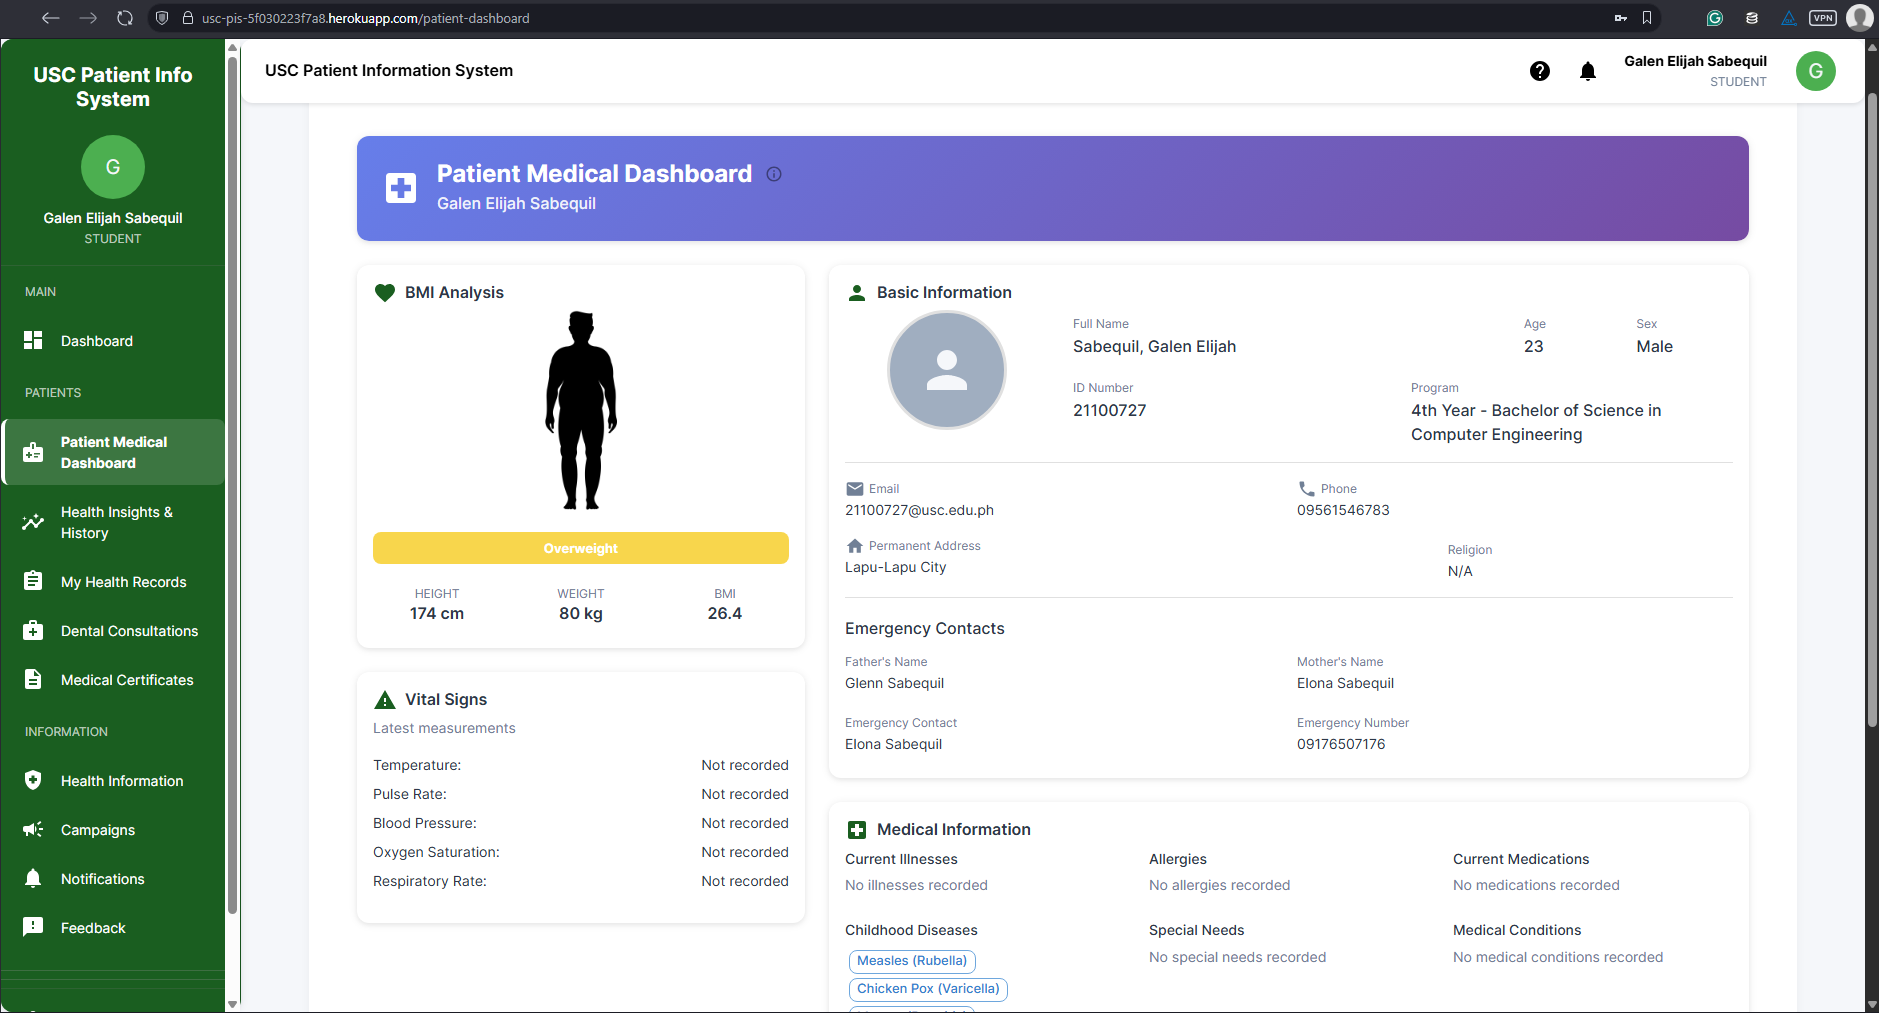
\includegraphics[width=1.1\textwidth]{StudentFacingPatientMedicalDashboard}}
    \caption{The Student-Facing Patient Medical Dashboard}
    \label{fig:student_dashboard}
\end{figure}

\subsection{Clinic Staff Management Interface}
The administrative interface prioritizes dense data processing and rapid retrieval. It features the newly engineered advanced filtering architecture, allowing staff to dynamically filter the patients list by Role, Program, Year Level, and Registration Period (Academic Year and Semester).

\begin{figure}[!ht]
    \centering
    \makebox[\textwidth][c]{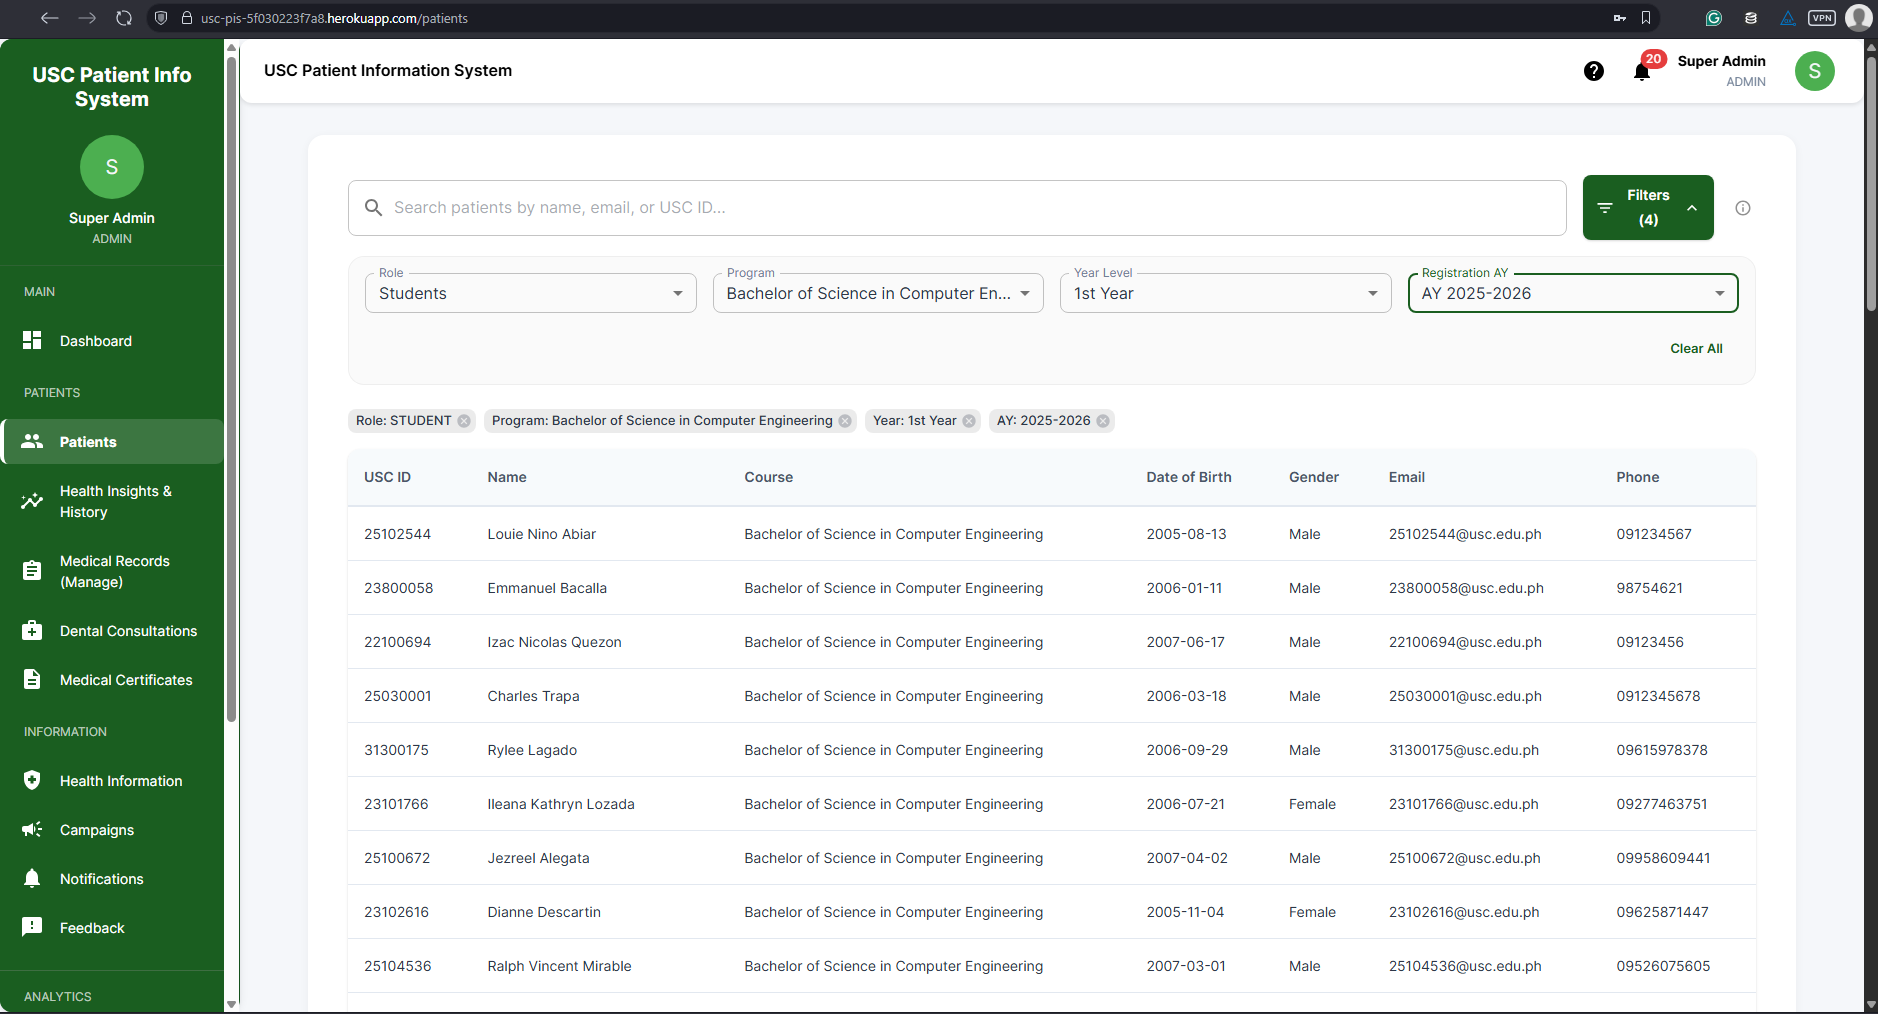
\includegraphics[width=1.1\textwidth]{StaffSidePatientList}}
    \caption{Clinic Staff Advanced Search/Filter Interface}
    \label{fig:staff_patient_list}
\end{figure}

\subsection{Health Awareness Campaign Feed}
The Health Information module acts as the clinic's digital bulletin board. This interface supports high-quality interactive image viewing (PubMats) and displays clinical alerts filtered strictly by active date ranges, eliminating cluttered or outdated announcements.

\begin{figure}[!ht]
    \centering
    \makebox[\textwidth][c]{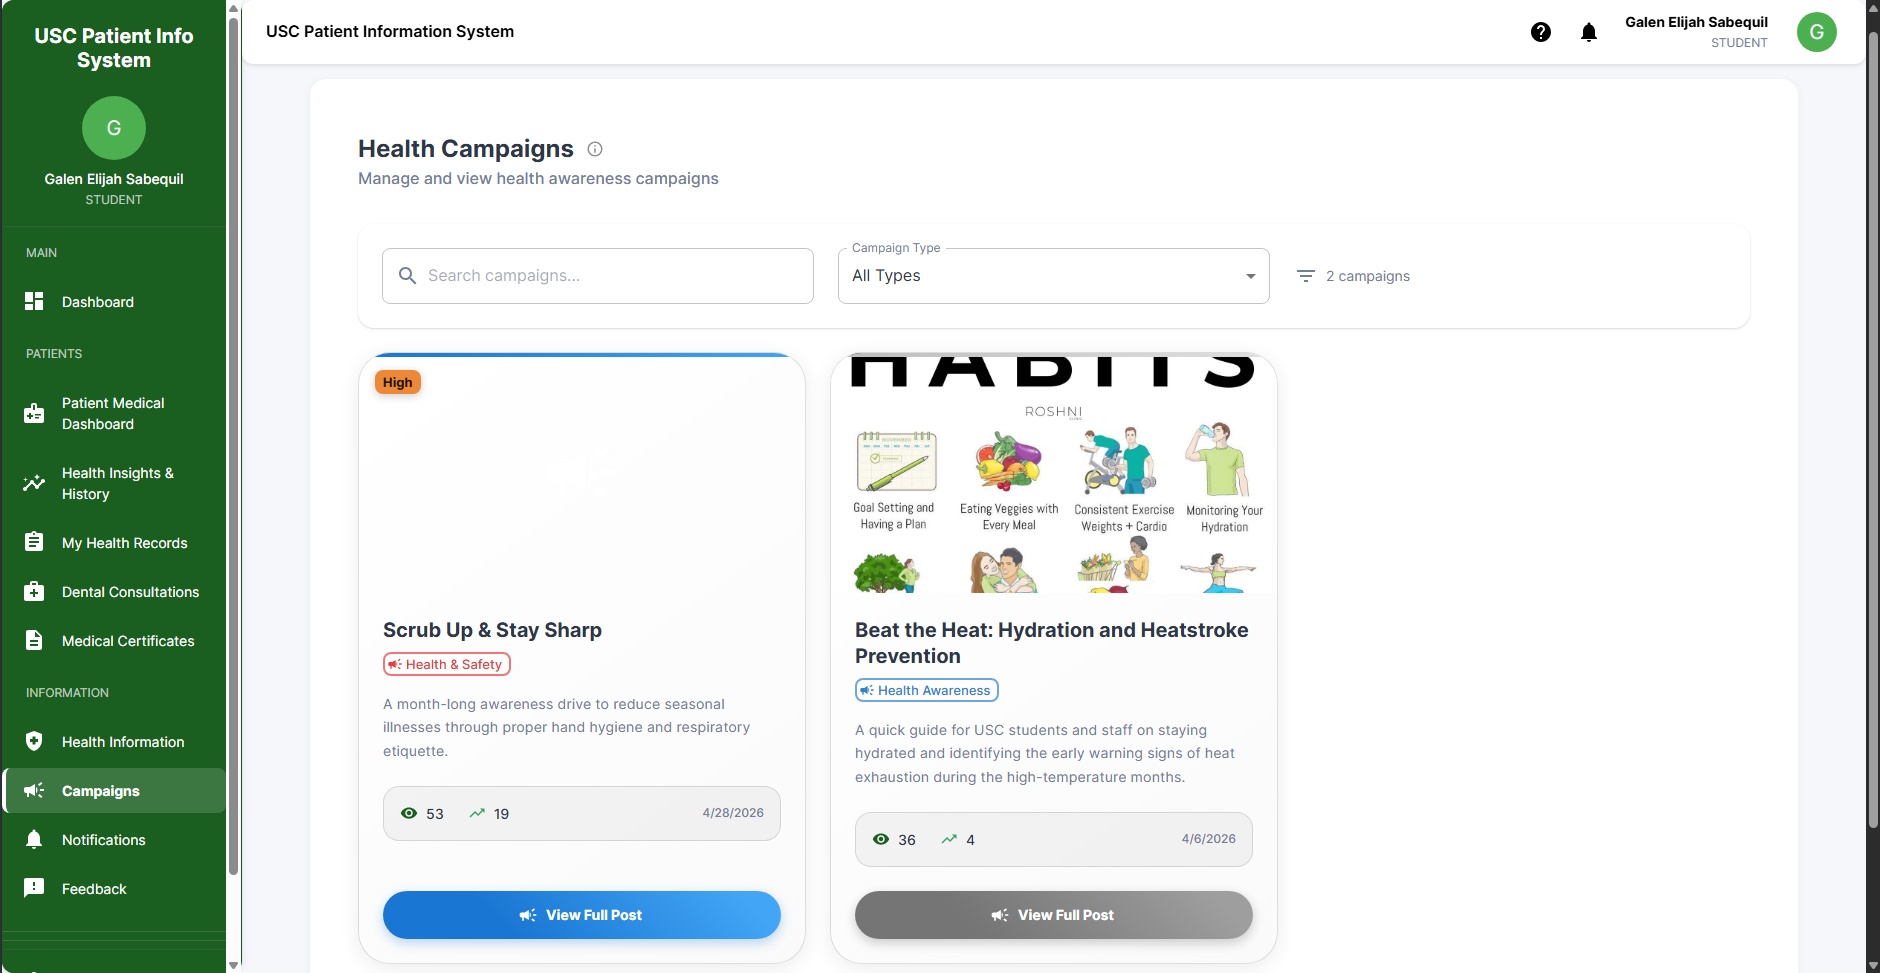
\includegraphics[width=1.1\textwidth]{StudentSideCampaignsFeed}}
    \caption{Health Awareness Campaign Student Feed}
    \label{fig:student_campaigns}
\end{figure}

\subsection{Medical Certificate Generation Preview}
The system's dual-engine PDF module autonomously generates the USC Form ACA-HSD-04F. The interface previews the landscape-formatted certificate, showcasing the automated mapping of the student's full course name, year level, and the Doctor's digital authorization.

\begin{figure}[!ht]
    \centering
    \makebox[\textwidth][c]{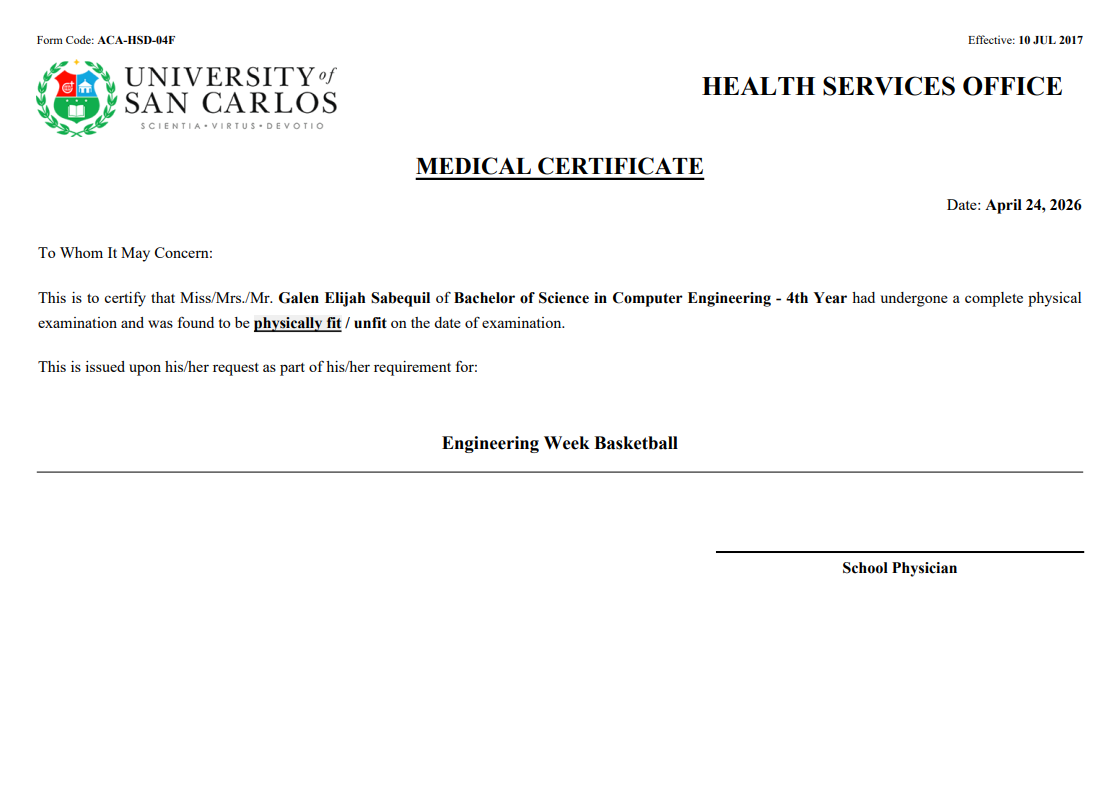
\includegraphics[width=1.1\textwidth]{Medical Certificate Generation Preview}}
    \caption{Generated Medical Certificate PDF Preview}
    \label{fig:med_cert_preview}
\end{figure}

\section{Data Privacy and Cryptographic Architecture}
Beyond basic role-gated access, the USC-PIS addresses the critical necessity of medico-legal documentation security. To safeguard Protected Health Information (PHI) and Personally Identifiable Information (PII), the system integrates advanced cryptographic measures at the database level. Utilizing the PostgreSQL \texttt{pgcrypto} extension, the platform enforces column-level symmetric encryption. All sensitive clinical inputs are instantly converted into secure \texttt{bytea} (BinaryField) hashes upon database commit, shielding plaintext data from unauthorized backend exposure. This ensures military-grade encryption-at-rest with an entirely negligible computational overhead of less than 1.0ms, allowing the clinic to maintain strict data privacy compliance without sacrificing system speed. To ensure absolute security, the symmetric AES-256 key is strictly managed via Heroku Environment Variables, ensuring it is never hardcoded into the GitHub repository or accessible via the source code. Furthermore, the file upload module implements stringent validation, rejecting high-risk executable formats (e.g., \texttt{.EXE}, \texttt{.JS}) to prevent malicious script injections.

\section{Entity Relationship Diagram (ERD) and Database Schema}
To ensure high data integrity, secure role-based access, and rapid query retrieval, the USC-PIS database is normalized and structured into highly interdependent relational tables. The Entity Relationship Diagram (ERD) illustrates the complete core architecture of the system, defining how user identities specialize into distinct profiles, and how clinical records and official certificates are securely mapped within the PostgreSQL environment.

\clearpage
\begin{sidewaysfigure}
    \centering
    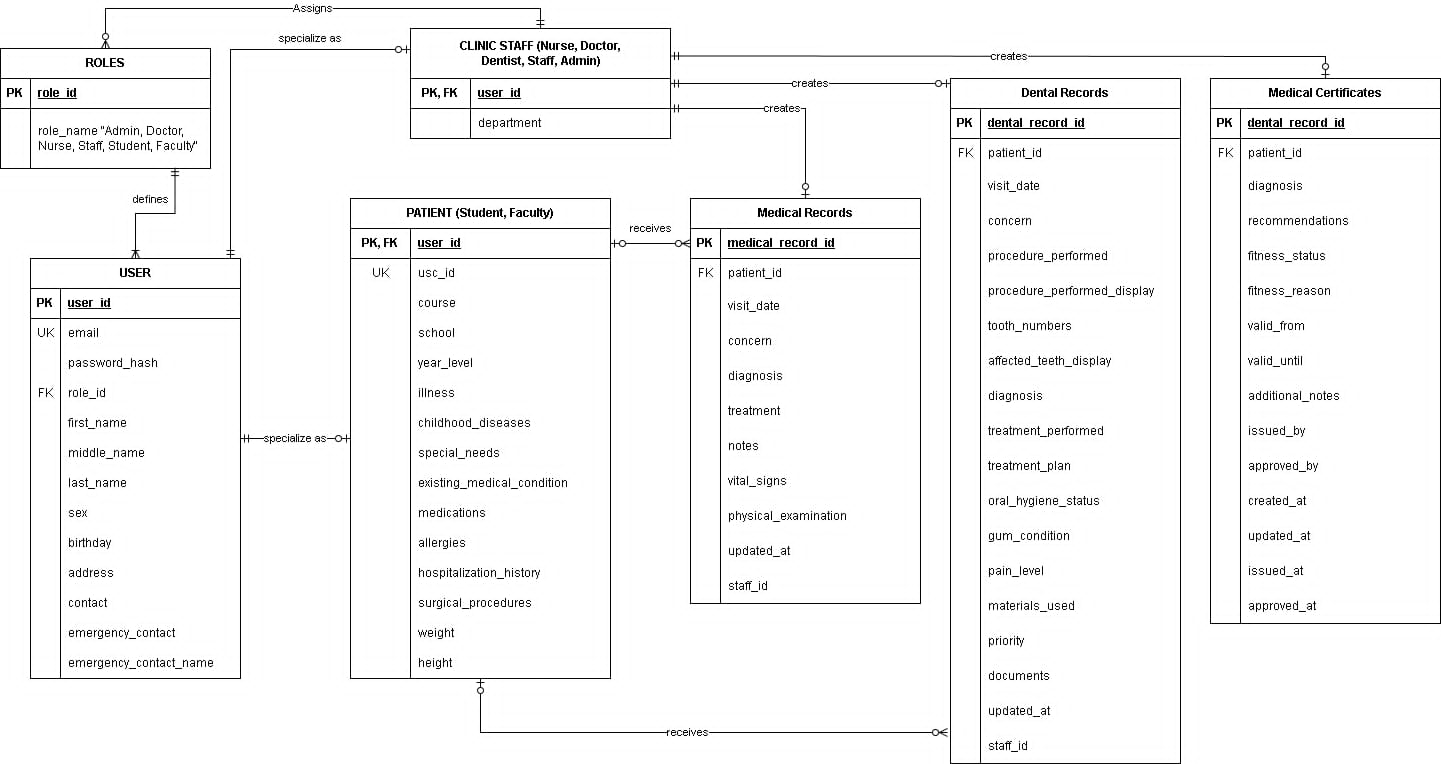
\includegraphics[width=1.0\textheight]{ERD_Final}
    \caption{Entity Relationship Diagram (ERD) of the USC-PIS}
    \label{fig:erd_final}
\end{sidewaysfigure}
\clearpage

\subsection{User Identity and Role Authorization}
The foundation of the system's architecture relies on the central \texttt{USER} entity, which stores core credentials such as the unique \texttt{email} (enforcing the Unique Key constraint), \texttt{password\_hash}, and foundational demographic data including \texttt{contact}, \texttt{address}, and \texttt{emergency\_contact\_name}. To enforce the system's strict Role-Based Access Control (RBAC) middleware, the \texttt{USER} table is directly linked via a Foreign Key (\texttt{role\_id}) to the \texttt{ROLES} entity. This table defines the absolute privileges of the account, specifically categorizing users as "Admin, Doctor, Nurse, Staff, Student, Faculty".

\subsection{Entity Specialization: Patients and Clinic Staff}
To eliminate data redundancy and cleanly separate clinical responsibilities, the database employs an entity specialization hierarchy. The base \texttt{USER} entity specializes into two distinct tables, utilizing \texttt{user\_id} as both a Primary Key and Foreign Key:

\begin{itemize}
    \item \textbf{CLINIC STAFF:} This table isolates medical personnel (Doctors, Nurses, Dentists, etc.) and associates them with their specific \texttt{department}. As illustrated in the schema, this entity holds the explicitly defined authority to "create" medical records, dental records, and certificates.
    \item \textbf{PATIENT:} This table captures extensive academic and medical metadata for students and faculty. It maps the unique \texttt{usc\_id}, \texttt{course}, \texttt{school}, and \texttt{year\_level}. Furthermore, it acts as a comprehensive health profile by tracking longitudinal data such as \texttt{childhood\_diseases}, \texttt{existing\_medical\_condition}, \texttt{surgical\_procedures}, \texttt{allergies}, and \texttt{medications}.
\end{itemize}

\subsection{Medical and Dental Record Management}
The core of the clinic's digital operations is handled by the \texttt{Medical Records} and \texttt{Dental Records} entities. The ERD explicitly illustrates that these records accumulate under a specific patient (via \texttt{patient\_id}) and are permanently audited to the staff member who created them (via \texttt{staff\_id}).

\begin{itemize}
    \item \textbf{Medical Records:} This entity tracks the \texttt{visit\_date}, chief concern, and the resulting \texttt{diagnosis} and \texttt{treatment}. It also features dedicated fields for comprehensive \texttt{vital\_signs}, \texttt{physical\_examination} inputs, and additional clinical notes. (\textit{Note: As detailed in Section 3.6, sensitive text payloads within these clinical fields are intercepted by backend signals and cryptographically hashed at rest using pgcrypto}).
    \item \textbf{Dental Records:} The dental entity is highly specialized to accommodate complex oral health charting. It captures specific clinical metrics including \texttt{oral\_hygiene\_status}, \texttt{gum\_condition}, \texttt{pain\_level}, and \texttt{materials\_used}. It also maps exact oral geography through the \texttt{tooth\_numbers} and \texttt{affected\_teeth\_display} fields, which restrict input to standard FDI notation boundaries.
\end{itemize}

\subsection{Medical Certificates and Administrative Workflows}
Crucially, the database schema seamlessly integrates the \texttt{Medical Certificates} entity to manage the digital issuance of the USC Form ACA-HSD-04F. This table is directly linked to the patient (\texttt{patient\_id}) and securely captures the \texttt{fitness\_status}, \texttt{fitness\_reason}, \texttt{diagnosis}, and \texttt{recommendations}. It also defines the exact validity timeframe via the \texttt{valid\_from} and \texttt{valid\_until} fields. To enforce strict clinical hierarchies and data integrity, the workflow is governed by two distinct tracking fields: \texttt{issued\_by} and \texttt{issued\_by\_doctor}. This schema constraint ensures that while clinical staff can draft and issue the initial document, an authorized Doctor must execute the final issuance (\texttt{issued\_at}) before the backend dual-engine PDF rendering is unlocked.

\section{Database Schema and Data Dictionary}
While the ERD visualizes the high-level entity relationships, the physical database schema dictates the strict data types, cryptographic boundaries, and structural constraints required for healthcare data management. The USC-PIS is normalized to eliminate data redundancy and ensure relationship integrity. The following data dictionaries outline the core tables powering the system's authentication and clinical operations.

\subsection{Identity and Authentication Schema}
The \texttt{authentication\_user} table serves as the core identity provider for the Role-Based Access Control (RBAC) middleware. To comply with data privacy protocols, sensitive health preconditions collected during registration are instantly encrypted into binary hashes.

\begin{table}[htbp]
\centering
\caption{Data Dictionary for authentication\_user}
\begin{tabular}{|l|l|p{7cm}|}
\hline
\textbf{Field Name} & \textbf{Data Type} & \textbf{Constraint / Description} \\
\hline
\texttt{id} & Integer & Primary Key (PK). Unique identifier for the user. \\
\hline
\texttt{email} & String (varchar) & Unique Key (UK). Enforces the \texttt{@usc.edu.ph} domain constraint. \\
\hline
\texttt{password} & String (varchar) & Securely hashed user password. \\
\hline
\texttt{role} & String (varchar) & RBAC identifier (ADMIN, DOCTOR, NURSE, DENTIST, STAFF, STUDENT). \\
\hline
\texttt{is\_verified} & Boolean & Flag indicating successful MFA OTP verification. \\
\hline
\texttt{illness\_enc} & BinaryField (bytea) & \texttt{pgcrypto} encrypted string of chronic illnesses. \\
\hline
\texttt{allergies\_enc} & BinaryField (bytea) & \texttt{pgcrypto} encrypted string of patient allergies. \\
\hline
\end{tabular}
\end{table}

\subsection{Clinical Profile Schema}
The \texttt{patients\_patient} table acts as the comprehensive demographic profile. It is logically decoupled from the authentication credentials to resolve over-normalization risks.

\begin{table}[htbp]
\centering
\caption{Data Dictionary for patients\_patient}
\begin{tabular}{|l|l|p{7cm}|}
\hline
\textbf{Field Name} & \textbf{Data Type} & \textbf{Constraint / Description} \\
\hline
\texttt{id} & Integer & Primary Key (PK). \\
\hline
\texttt{user\_id} & Integer & Foreign Key (FK) mapping to \texttt{authentication\_user.id}. \\
\hline
\texttt{usc\_id} & String (varchar) & 8-digit official University ID number. \\
\hline
\texttt{academic\_year} & String (varchar) & Retooling filter field (e.g., 2025-2026) for cohort isolation. \\
\hline
\texttt{first\_name\_enc} & BinaryField (bytea) & \texttt{pgcrypto} encrypted first name payload. \\
\hline
\texttt{last\_name\_enc} & BinaryField (bytea) & \texttt{pgcrypto} encrypted last name payload. \\
\hline
\texttt{created\_at} & Datetime & Immutable audit trail timestamp for record creation. \\
\hline
\end{tabular}
\end{table}

\subsection{Clinical Records Schema}
The \texttt{patients\_medicalrecord} and \texttt{patients\_dentalrecord} tables capture the specialized clinical data. These tables enforce rigorous validation, such as JSON structuring for vitals and regex validation for FDI dental notation.

\begin{table}[htbp]
\centering
\caption{Data Dictionary for patients\_medicalrecord}
\begin{tabular}{|l|l|p{7cm}|}
\hline
\textbf{Field Name} & \textbf{Data Type} & \textbf{Constraint / Description} \\
\hline
\texttt{id} & Integer & Primary Key (PK). \\
\hline
\texttt{patient\_id} & Integer & Foreign Key (FK) mapping to \texttt{patients\_patient.id}. \\
\hline
\texttt{created\_by\_id} & Integer & Foreign Key (FK) mapping to the attending medical staff's \texttt{user\_id}. \\
\hline
\texttt{concern} & String (varchar) & Mandatory chief complaint or reason for clinical visit. \\
\hline
\texttt{diagnosis\_enc} & BinaryField (bytea) & \texttt{pgcrypto} encrypted clinical diagnosis payload. \\
\hline
\texttt{vital\_signs} & JSON & Structured JSON array capturing BP, HR, Temp, and SpO2. \\
\hline
\end{tabular}
\end{table}

\begin{table}[htbp]
\centering
\caption{Data Dictionary for patients\_dentalrecord}
\begin{tabular}{|l|l|p{7cm}|}
\hline
\textbf{Field Name} & \textbf{Data Type} & \textbf{Constraint / Description} \\
\hline
\texttt{id} & Integer & Primary Key (PK). \\
\hline
\texttt{patient\_id} & Integer & Foreign Key (FK) mapping to \texttt{patients\_patient.id}. \\
\hline
\texttt{tooth\_numbers} & String (varchar) & CSV string of affected teeth enforcing FDI Notation (11-48) limits. \\
\hline
\texttt{procedure\_performed} & String (varchar) & Defined choices constraint (e.g., CLEANING, EXTRACTION). \\
\hline
\texttt{tooth\_chart} & JSON & Structured representation of the visual dental diagram. \\
\hline
\end{tabular}
\end{table}

\subsection{Administrative Workflow Schema}
The \texttt{medical\_certificates} table manages the End-to-End issuance of the USC Form ACA-HSD-04F. It utilizes dual Foreign Keys to track both the staff member who drafted the document and the Doctor who finalized it.

\begin{table}[htbp]
\centering
\caption{Data Dictionary for medical\_certificates}
\begin{tabular}{|l|l|p{7cm}|}
\hline
\textbf{Field Name} & \textbf{Data Type} & \textbf{Constraint / Description} \\
\hline
\texttt{id} & Integer & Primary Key (PK). \\
\hline
\texttt{patient\_id} & Integer & Foreign Key (FK) mapping to \texttt{patients\_patient.id}. \\
\hline
\texttt{fitness\_status} & String (varchar) & Constrained to choices: 'physically fit' or 'unfit'. \\
\hline
\texttt{approval\_status} & String (varchar) & Tracks document state: 'draft', 'pending', 'issued', 'rejected'. \\
\hline
\texttt{issued\_by} & Integer & Foreign Key (FK) mapping to the Nurse/Staff who drafted the form. \\
\hline
\texttt{issued\_by\_doctor} & Integer & Foreign Key (FK) mapping strictly to an authorized Doctor. \\
\hline
\end{tabular}
\end{table}

\section{Network Configuration and Deployment Architecture}
To guarantee high availability and real-time synchronization between the clinic staff and student users, the USC-PIS utilizes a robust cloud-based deployment architecture. The infrastructure is specifically configured to handle enterprise-level healthcare operations, leveraging several cloud services to manage hosting, media delivery, and secure communications.

\subsection{CI/CD Pipeline and Cloud Hosting}
The application is hosted on Heroku, which serves as the primary deployment platform for the backend Application Layer. To ensure that no critical bugs or security vulnerabilities enter the production environment, the deployment process utilizes a Continuous Integration and Continuous Deployment (CI/CD) pipeline engineered via GitHub Actions. This automated DevOps pipeline mandates that all code commits must successfully pass 15 rigorous automated tests—ranging from unit tests (UT-01 to UT-06) to integration and performance tests (PT-01 to PT-04)—before the system permits the build to be deployed to the live Heroku dynos.

\subsection{Dual-Database Environment}
The system employs a dual-database paradigm to balance rapid development with secure production data handling. During local testing and development, the system utilizes SQLite to allow for lightweight operations. However, the live production environment is powered by a PostgreSQL 16.8 server hosted on Heroku. To prevent crashes between the two environments, "Vendor-Aware" logic is implemented within the system's backend migrations, ensuring that PostgreSQL-exclusive functions (such as \texttt{pgcrypto} cryptographic extensions) are safely bypassed in the local environment but strictly enforced in the cloud.

\subsection{Scalable Content Delivery Network (CDN)}
Due to the significant file storage requirements of digital health records, including PubMats, campaign banners, and PDF attachments, the system offloads media storage from the primary database. Cloudinary is integrated as a scalable Content Delivery Network (CDN) to manage these file uploads natively. By offloading media processing to Cloudinary, the primary Django application is relieved of heavy bandwidth tasks, ensuring the HTTP threads remain unblocked and patient data loads seamlessly across devices.

\subsection{Secure Communications Integration}
To automate clinic communications such as verification codes, patient feedback reminders, and password resets, the system interfaces directly with the Gmail API. Instead of relying on traditional SMTP configurations, which are prone to being flagged by strict firewall policies, the USC-PIS implements an OAuth 2.0 protocol. This ensures reliable, uninterrupted delivery of automated clinic alerts directly to the students' \texttt{@usc.edu.ph} institutional inboxes.

\section{Development and Testing Strategy}

The development adhered to an Agile methodology, ensuring iterative cycles that adapted to clinical staff feedback. To ensure software quality and alignment with functional requirements, the system underwent a rigorous, multi-layered testing pipeline.

\subsection{Functional and Security Testing}

\begin{itemize}
    \item \textbf{Unit Testing (UT-01 to UT-06):} Validated isolated components and logic constraints. Key tests verified the strict binary storage of \texttt{pgcrypto} encrypted data, accurate regex enforcement of the FDI 11-48 dental record range, and the rejection of \texttt{.EXE} and \texttt{.JS} file uploads to secure system integrity.
    \item \textbf{Integration Testing (IT-01 to IT-05):} Evaluated end-to-end interactions between the frontend, backend, and external APIs. This included simulating the end-to-end medical certificate pipeline (from a Nurse's draft to a Doctor's issuance to PDF rendering) and executing RBAC stress tests to ensure unauthorized users could not bypass role-gated endpoints.
\end{itemize}

\subsection{Performance Testing}

Quantitative benchmarks evaluated the system's operational capability to handle peak clinical loads (PT-01 to PT-04).

\begin{itemize}
    \item \textbf{Search Efficiency:} Patient search query latency was successfully recorded between 123.16ms and 127.81ms, functioning nearly four times faster than the 500ms maximum threshold.
    \item \textbf{PDF Generation:} The dual-engine PDF module consistently generated official Medical Certificates in 122.93ms to 124.53ms.
    \item \textbf{Concurrency:} The architecture stabilized processing 20 simultaneous HTTP requests in 0.66 seconds with a 0\% data drop rate.
\end{itemize}

\subsection{User Acceptance Testing (UAT)}

Preliminary User Acceptance Testing (UAT) was conducted to measure the system's usability and feature relevance.

\begin{itemize}
    \item \textbf{Staff Evaluation:} Nurses, Doctors, and Dentists noted strong efficiency improvements over legacy operations, citing that generating data was significantly easier. Feedback from this group, alongside exhaustive panel recommendations, directly resulted in the comprehensive ``Application Retooling'' phase. This critical iteration involved: (1) engineering the advanced filter bar to segment patient lists dynamically by Academic Year; (2) implementing the Attributed Clinical Remarks system to ensure Doctors can view observations from other medical personnel; and (3) completely reworking the asynchronous reporting engine to support interactive charts and landscape layouts, among other strategic architectural enhancements.
    \item \textbf{Student Evaluation:} UAT was conducted with the student demographic to evaluate accessibility. Based on the responses, the system received overwhelmingly positive feedback, with users praising the Patient Medical Dashboard and automated BMI calculations. Constructive feedback included a request for a ``Dark Mode'' toggle and improved mobile responsiveness.
\end{itemize}

\section{Validation and Pilot Deployment}

To guarantee a smooth transition from a paper-based system to the fully digital USC-PIS, the deployment will follow a highly structured roll-out.

\subsection{Pilot Deployment}

The initial pilot deployment exclusively targeted 70 out of the 99 enrolled students (approximately 71\%) currently enrolled in CPE 1202L (Data Structures and Algorithms), resulting in a student sample size of N=70, alongside selected clinical staff. This targeted demographic offers a representative sample size to accurately validate data synchronization, performance thresholds, and operational workflows under real clinic loads before expanding the system to the entire university.

\subsection{Training and Support}

To equip the clinic personnel with the necessary digital competency, training will be executed via a hybrid approach utilizing hands-on demonstration modules supplemented by comprehensive User Manuals.

\begin{itemize}
    \item \textbf{Role-Specific Modules:} Nurses will be trained to utilize the Retooling Filter Bar to segment patient datasets via Academic Year logic. Dentists will be trained to optimize high-volume clinic days by utilizing the streamlined ``Consultation Only'' mode. Administrative Staff will be trained on the asynchronous Celery-powered reporting module and the strict RBAC constraints mandated for Medical Certificate issuance.
\end{itemize}

\subsection{Secondary Comparative Simulation}

To fulfill additional requirements from the evaluation committee, a second phase of hands-on simulations was conducted. This secondary simulation involved N=30 students who possessed prior experience with the legacy manual clinic processes, along with N=8 clinic staff members. Participants actively utilized the latest system workflows, providing a direct operational comparison between the digital USC-PIS and the legacy manual paper-based methods.

To ensure a comprehensive evaluation of the patient-facing features, the student simulation was highly structured. Participants were instructed to: (1) Register and authenticate using their \url{@usc.edu.ph} email via the automated OTP system; (2) Navigate their personalized Patient Medical Dashboard to view their automated BMI and vital signs; (3) Access the Health Campaigns feed to view interactive PubMats and educational materials; (4) Simulate the end-to-end process of requesting a medical certificate; (5) Check for timely in-app and email notifications; and (6) Test the automated digital feedback system by rating their simulated visit.

The clinic staff simulation was designed to test heavy administrative and clinical workflows. Nurses, Doctors, and Dentists were instructed to: (1) Utilize the advanced filtering architecture to search and isolate patient records by academic year and semester; (2) Create and update mock medical and dental records, specifically testing the newly integrated ``Attributed Clinical Remarks'' feature where doctors view peer notes; (3) Process a simulated medical certificate from the initial nurse draft to the final doctor authorization and PDF rendering; (4) Manage the posting of health awareness campaigns; and (5) Utilize the asynchronous reporting engine to generate formatted medical and statistical reports. 

Following the simulation, a dual-survey methodology was employed. First, the original general usability survey was re-administered to confirm that the system remained intuitive following the ``Application Retooling'' phase. Second, a new, targeted comparative evaluation form was deployed to explicitly measure the digital system's operational upgrade against the legacy manual baseline. This two-pronged approach ensures both core usability and objective attainment are mathematically proven. Only after executing these specific tasks were the staff allowed to evaluate the web-based system against their manual baseline.

